%
% chapter.tex
%
% (c) 2020 Prof Dr Andreas Müller
%
\chapter{Berechnung
\label{chapter:berechnung}}
\lhead{Berechnung}
\rhead{}
Die numerischen Datentypen eines digitalen Computers sind Approximationen
für die abstrakten Zahlensysteme $\mathbb{N}$, $\mathbb{Z}$, $\mathbb{Q}$
und $\mathbb{R}$.
Man kann sie daher verwenden, die in der Analysis und der linaren Algebra
definierten Konzepte wie Grenzwerte, Integrale oder inverse Matrizen zu
berechnen.
Da sie jedoch nur Annäherungen sind, werden die gewohnten Rechenregeln 
nicht immer gültig sein.
In $\mathbb{R}$ kann die Addition dreier Zahlen zum Beispiel in beliebiger
Reihenfolge durchgeführt werden, für \texttt{double}-Zahlen auf einem
Computer ist dies nicht der Fall.
Zum Beispiel kann man in Octave die folgende Rechnung durchführen\footnote{%
Das Beispiel zeigt eine Problem für Zahlen vom Typ \texttt{double}.
Das Programm \texttt{assoziativ.cpp} im Verzeichnis
\texttt{buch/chapters/experiments/assoziativ} findet analoge Beispiel für
die anderen Floatingpoint Typen \texttt{float} und \texttt{long double}.}:
\verbatiminput{chapters/10-arithmetik/assoziativ.txt}
Das Assoziativgesetz verlangt, dass $a+(b+b)=(a+b)+b$ ist und zunächst
will es auch den Anschein haben, dass $x$ und $y$ tatsächlich gleich sind.
Ungewöhnlich ist nur, dass der Wert von $x$ mit auf den ersten Blick
unnötigen Nachkommastellen angezeigt wird.
Diese Nullen deuten jedoch an, dass $x\ne 1$ aber $y=1$, man in Schritt
6 und 7 sieht, wenn man die Differenz zu $1$ bestimmt.

Das Beispiel verdeutlicht, dass auf einem Computer zur Verfügung
stehende numerische Datentypen die gewohnten Rechengesetze verletzen und
neue Unzulänglichkeiten wie Rundungsfehler in die Berechnung injizieren.
Die Numerik muss sich daher mit der Frage befassen, welcher Art diese
neuen Effekte sind und wie ihnen effektiv begegnet werden kann.
Nur so kann die Zuverlässigkeit numerisch gefundener Resultate
garantiert werden.

Dieses Kapitel befasst sich mit den Eigenschaften von Computer-Zahlensystemen.
Im ersten Abschnitt werden die Zahlensysteme beschrieben und ihre 
Vor- und Nachteile gegeneinander abgewogen.
Im zweiten Abschnitt wird gezeigt, wie Resultate bei unvorsichtiger
Vorgehensweise verfälscht werden können.
Rundungsfehler sind unvermeidlich, das Ziel muss daher sein, ihre
Grösse unter Kontrolle zu halten.
Numerische Instabilität liegt vor, wenn die Berechnung aufgrund von
numerischen Effekten völlig aus dem Ruder läuft und sinnlose Resultate
liefert, dies wird in Abschnitt~\ref{buch:section:instabilitaet}
untersucht.


%
% zahlensysteme.tex
%
% (c) 2020 Prof Dr Andreas Müller, Hochschule Rapperswil
%
\section{Zahlensysteme
\label{buch:section:zahlensysteme}}
\rhead{Zahlensysteme}
Auf modernen Allzweck-Prozessoren steht eine ganze Reihe verschiedener
numerischer Datentypen mit unterschiedlichen Eigenschaften
bezüglich Geschwindigkeit und Fehlerverhalten zur Verfügung.
In diesem Abschnitt sollen sie vorgestellt und miteinander verglichen
werden.
Es gilt, den für eine Berechnung zweckmässigsten Typen zu wählen,
wobei Speicherbedarf, Laufzeit und Parallelisierbarkeit wesentliche
Aspekte sind.

Microcontroller sind im Vergleich zu Allzweckprozessoren oft stark
\index{Microcontroller}%
eingeschränkt.
Meist sind nur Ganzahltypen mit oft sehr beschränkter Länge implementiert.
Manchmal kann die Arithmetik-Einheit des Prozessors nicht einmal eine
Multiplikation in Hardware ausführen, sie muss in Software zeitaufwendig
nachgebildet werden.
Für Floatingpoint-Operationen muss oft Bibliotheken zurückgegriffen
werden, die den Speicherbedarf erhöhen und langsam sind.
Die Implementation von numerischen Berechnungen in eingebetteten Anwendungen
ist daher mit besonderen Herausforderungen konfrontiert.

Dieselbe Schwierigkeit haben auch Allzweck-Prozessoren, wenn die
Genauigkeitsanforderungen die Möglichkeiten der von der Prozessor-Hardware
implementierten Typen übersteigt.
Dieser Fall tritt beispielsweise bei Berechnungen in der Kryptographie auf,
wo oft mit Ganzzahlen mit Tausenden von Stellen gerechnet werden muss.
Im Abschnitt~\ref{buch:subsection:mp} mit der GNU Multiprecision-Library
ein Beispiel einer solchen Bibliothek vorgestellt.

%
% Zahlendarstellung bezüglich verschiedener Basen
%
\subsection{Zahlendarstellung bezüglich verschiedener Basen
\label{buch:subsection:basen}}
Allen Zahlensystemen gemeinsam ist die Positionsdarstellung.
\index{Positionsdarstellung}
Eine Zahl wird als Zeichenkette $x=x_nx_{n-1}\dots x_3x_2x_1x_0$
geschreiben,
wobei die Zeichen $x_i$ Ziffern mit $0 \le x_i < b$ sind.
$b$ ist die Basis des Zahlensystems.
Der Wert der Zahl $x$ ist dann 
\[
x
=
\sum_{k=1}^n x_kb^k.
\]
Um die Basis deutlich zu machen, 
hängen wir die Basis also Index an eine Zahlendarstellung an.
Es ist also zum Beispiel
\[
1291_{10}
=
10100001011_2
=
1202211_3
=
2413_8
=
508_{16}.
\]
Bruchzahlen können analog dargestellt werden.
Die Zeichenkette
\[
x = x_{n}x_{n-1}\dots x_2x_1x_0\texttt{.}x_{-1}x_{-2}x_{-3}\dots x_{-m}\dots
\]
hat den Wert
\[
x = \sum_{k=-m}^n x_kb^k.
\]
Die Zahl $\pi$ hat daher die Darstellungen
\begin{align*}
\pi
&=
11.0010010000111111011011_2
\\
&=
10.01021101222201_3
\\
&=
3.11037552_8
\\
&=
3.1415926_{10}
\\
&=
3.243F6A_{16}
\end{align*}
in den Basen $2$, $3$, $8$, $10$ und $16$.
Eine grössere Basis erlaubt zwar eine kompaktere Darstellung, aber
für die Rechnung ermöglicht die binäre Darstellung die einfachste
und damit auch schnellste Implementation.

Man beachte, dass endliche Dezimalbrüche in anderen Basen durchaus
nicht mehr endlich zu sein brauchen.
So ist zum Beispiel
\begin{align*}
\frac12&= 0.5_{10} = 0.1_{2},
\\
\frac15&= 0.2_{10} = 0.001100110011\dots = 0.\overline{0011}_{2},
\\
\frac13&= 0.\overline{3}_{10} = 0.\overline{01}_{2}.
\end{align*}
Eine Konsequenz dieser Beobachtung ist, dass nur schon die Umwandlung
einer Dezimalzahl ins Binärsystem und die Rückumwandlung in eine Dezimalzahl
den Wert verändern kann.
Zum Beispiel\footnote{Dieses Beispiel wurde mit dem Programm
\texttt{format.cpp} aus dem Verzeichnis
\texttt{buch/chapters/experiments/limits} von \cite{buch:repo}
gerechnet.}
bewirkt der C++-Code
\begin{verbatim}
double	x = 0.2;
std::cout << x;
\end{verbatim}
dass der Compiler zunächst die Dezimalzahl $0.2$ in eine Binärzahl
verwandelt, diese Form wird im ausführbaren Code gespeichert.
Zur Laufzeit des Programms muss die I/O-Bibliothek dann die gespeicherte
Zahl wieder in eine Dezimalzahl verwandeln.
Für $x=0.5$ wäre das unproblematisch, da diese Zahl sowohl dezimal wie
auch binär ein endlicher Dezimalbruch ist.
Für $x=0.2$ tritt jedoch eine Abweichung auf, weil die im Code gespeichert
Binärzahl nicht exakt in $0.2$ zurückgewandelt werden kann.
Stattdessen erhält man abhängig vom Datentyp die abweichenden
Werte von Tabelle~\ref{buch:zahlensysteme:rundung}.
\begin{table}
\centering
\begin{tabular}{|>{\tt}r|>{$}r<{$}|>{$}r<{$}|}
\hline
\textrm{Typ}& 0.5\phantom{0000000000000000000}
                                    & 0.2\phantom{0000000000000000000}\\
\hline
float       & 0.50000000000000000000& 0.20000000298023223877\\
double      & 0.50000000000000000000& 0.20000000000000001110\\
long double & 0.50000000000000000000& 0.20000000000000001110\\
\hline
\end{tabular}
\caption{Nicht alle exakt darstellbaren Dezimalzahlen sind auch im
Binärsystem exakt darstellbar.
Die Zahl $0.2_{10}$ führt auf einee periodischee Binärzahl, die
beim abspeichern gerundet werden muss.
Je nach Datentyp weicht der gerundete Wert mehr oder weniger stark ab.
\label{buch:zahlensysteme:rundung}}
\end{table}
Dass kein Unterschied zwischen \texttt{double} und \texttt{long double}
besteht, ist nur scheinbar. 
Multipliziert man $x$ mit $5$ vor dem Output, wird plötzlich ein
Unterschied sichtbar.

%
% Festkommazahlen
%
\subsection{Festkommazahlen
\label{buch:subsection:integers}}
Die bekanntesten Festkommazahlen sind die Ganzzahltypen, die jeder
Prozessor zum Beispiel für Adressierung, Zähler und Indizierung
benötigt.
Damit ist auch bereits klar, dass man immer damit rechnen kann, dass
mindestens die Addition und die Subtraktion von ganzen Zahlen mit
Wortlängen implementiert sind, die der Prozessor zum Beispiel für
relative Adressierung braucht.
Ebenso kann man davon ausgehen, dass jeder Kern eines Prozessors
eine Einheit für ganzzahlige Operationen hat, denn er könnte sonst
nicht einmal die minimal notwendigen Adressberechnungen durchführen.

\subsubsection{Addition}
Das Verfahren der ``schriftlichen Addition'', welches man in der Primarschule
lernt, funktioniert auch für die Berechnung einer Summe in jeder beliebigen
anderen Basis.

\subsubsection{Vorzeichen}
Ganzzahlen mit Vorzeichen können auf verschiedene Arten binär dargestellt
werden, weitgehend durchgesetzt hat sich für Festkommazahlen jedoch die
Zweierkomplement-Darstellung\footnote{Der Exponent einer Gleitkommanzahl
ist zwar auch eine Ganzzahl, er wird aber gemäss Standard IEEE 754
nach einem anderen Verfahren codiert, siehe dazu auch
Abschnitt~\ref{buch:subsection:floatinpoing}}.
In ihr werden 8-bit Zeichenketten wie folgt als Zahlen interpretiert:
\begin{align*}
\texttt{01111111}&= \phantom{-}127\\
\texttt{01111110}&= \phantom{-}126\\
\vdots\quad&\qquad\vdots\\
\texttt{00000010}&= \phantom{-00}2\\
\texttt{00000001}&= \phantom{-00}1\\
\texttt{00000000}&= \phantom{-00}0\\
\texttt{11111111}&= -\phantom{00}1\\
\texttt{11111110}&= -\phantom{00}2\\
\texttt{11111101}&= -\phantom{00}3\\
\vdots\quad&\qquad\vdots\\
\texttt{10000010}&=-126\\
\texttt{10000001}&=-127\\
\texttt{10000000}&=-128
\end{align*}
Diese Codierung ist in Hardware besonders leicht implementiertbar.
Ein Zähler für eine Vorzeichenlose Ganzzahl von 8 bit Länge, initialisiert
mit \texttt{10000000} wird beim Hochzählen genau die Zahlen von $-128$
bis $127$ aufzählen.

Die Entgegengesetzte einer Zahl kann nach der folgenden Regel gefunden werden:
\begin{enumerate}
\item Man nehme das Komplement jedes einzelnen Bits einer Zahl
\item Addiere 1.
\end{enumerate}
\begin{beispiel}
Die Zahl $-1291$ soll als 16-bit Ganzzahl in Zweier-Komplement-Darstellung
geschrieben werden.
Zunächst wird die Binärdarstellung benötigt:
$1291_{10}= \texttt{0000010100001011}_2$.
\begin{enumerate}
\item Bits komplementieren: \texttt{1111101011110100}
\item $1$ addieren: \texttt{1111101011110101}
\qedhere
\end{enumerate}
\end{beispiel}

Die Addition vorzeichenbehafteter Ganzzahlen funktioniert für die
Zweierkomplementdarstellung nach dem bekannten Algorithmus für die
Addition.
Die Differenz $111-88$ kann man als Summe $111+(-88)$ schreiben.
Als 8-bit Binärzahlen sind die beiden Operanden
\texttt{01101111} und \texttt{10101000}.
Ihre Summe ist
\begin{center}
\begin{tabular}{>{\tt}r}
01101111\\
10101000\\
\hline
{\color{gray}}\,
00010111\\
\end{tabular}
\end{center}
Dabei ist zwar ein Überlauf aufgetreten, aber dieser kann ignoriert
werden.
Tatsächlich ist $23_{10}=10111_2$.
Der grosse Vorteil dieser Vorzeichenkonvention ist also, dass
für die Addition vorzeichenbehafteter Ganzzahlen in
Zweierkomplement-Darstellung die gleiche vorhandene Hardware verwendet
werden kann wie für die Addition vorzeichenloser Ganzzahlen.

\subsubsection{Multiplikation und Division}
Man kann allerdings nicht davon ausgehen, dass ein Prozessor auch
die Multiplikation von ganzen Zahlen und erst recht die Division
von ganzen Zahlen implementiert.
In den meisten Fällen benötigt der Prozessor nur die Multiplikation
mit kleinen Zweierpotenzen, die sich viel effizienter als
Verschiebeoperationen durchführen lassen.

\subsubsection{Nachkommateil}
Bisher wurden ausschliesslich Ganzzahlen betrachtet.
Man kann diese Ganzzahlen aber auch als rationale Zahlen mit einem
Nachkommateil fester Länge betrachten.
Man könnte sich zum Beispiel nach den ersten 8 bit einer 16-bit Zahl
ein Komma denken und die nachfolgenden Bits als Bruchteil
betrachten.
Die Bitfolge \texttt{0000000110010000} muss dann als
\[
00000011.00100000_2
=
3.125_{10}
\]
interpretiert werden.
An den Algorithmen für Addition und Subtraktion ändert sich nichts,
es ist daher keine neue Hardware für die Implementation dieser
Operationen notwendig, die Ganzzahloperationen reichen aus.

Etwas komplizierter ist die Sache bei der Multiplikation.
Nehmen wir an, dass wir mit 8-bit Festkomma-Zahlen arbeiten mit
einem Nachkommateil von 4 bits. 
Wir möchten das Produkt $3.125\cdot 2.0625$ berechnen.
Die Binärdarstellungen dieser Zahlen sind
$3.125_{10}=11.001_{2}$ und $2.0625_{10}= 10.0001_{2}$.
Das Produkt der 8-bit Ganzzahlen \texttt{00110010} und \texttt{00100001}
wird mehr Platz beanspruchen, im schlimmsten Fall 16 bit:
\[
\texttt{00110010}_2\cdot\texttt{00100001}_2
=
\texttt{0000011001110010}_2.
\]
In den Faktoren sind die letzten 4 Stellen jeweils als Nachkommateil
zu unterpretieren, also sind im Produkt die letzten 8 Stellen als
Nachkommateil zu interpretieren.
Das Produkt, wieder als 8-bit Festkommazahl geschrieben ist daher
\[
\texttt{0011.0010}_2\cdot\texttt{0010.0001}_2
=
\texttt{00000110.01110010}_2
\approx
\texttt{0110.0111}_2
\]
Auch für die Multiplikation ist keine neue Hardware erforderlich,
doch muss das Resultat entsprechend mit Schiebeoperationen wieder
so formattiert werden, dass das Komma an der ``richtigen'' Stelle
landet.

Mit den Ganzzahl-Operationen einer CPU lassen sich also auch sehr
schnelle Festkomma-Ope\-ra\-tio\-nen realisieren.

\subsubsection{Vor- und Nachteile von Festkommazahlen}
\begin{itemize}
\item[$\oplus$]
Eine beliebige relle Zahl muss bei der Darstellung als Festkommazahl
um Maximal die Hälfte der Wertigkeit der letzten Stelle gerundet werden.
Dieser absolute Fehler ist konstant.
\item[$\oplus$]
Operationen sind typischerweise deutlich schneller als
mit Gleitkommazahlen vergleichbarer Grösse.
Dies gilt insbesondere dann, wenn die Operationen zum Teil in Software 
realisiert werden müssen.
\item[$\oplus$] Die Addition und Subtraktion sind von derart elementarer
Bedeutung für einen CPU-Kern, dass jeder Kern mindestens eine Einheit
für Ganzzahl-Operationen hat.
In einer Multicore-CPU kann man daher davon ausgehen, dass Festkomma-Operationen
sich auf verschiedenen Cores nicht gegenseitig behindern.
\item[$\ominus$] Kleine Zahlen können nur mit wenigen signifikanten
Stellen dargestellt werden.
\item[$\ominus$] Schon für mässig grosse Zahlen ist Überlauf möglich.
\end{itemize}

%
% Gleitkommazahlen
%
\subsection{Gleitkommazahlen
\label{buch:subsection:floatinpoing}}
Gleitkommazahlen erweitern den Bereich der darstellbaren Zahlen dadurch,
dass sie zu einer Festkommazahl einen Exponentialfaktor hinzunehmen.
Eine Gleitkommazahl $x$ ist also von der Form
\[
x = m \cdot b^k.
\]
$m$ heisst Mantisse, $b$ ist die Basis und $k$ ist der
Exponent, üblicherweise eine kleine Ganzzahl.
Die Mantisse wird typischerweise so strukturiert, dass genau eine 
Stelle vor dem Komma steht.
Im Dezimalsystem sind also
\[
1291
=
1.291\cdot 10^{3},
\quad
\gamma = 5.772156649\cdot 10^{-1},
\quad
N_A
=
6.0221476\cdot 10^{23}
\]
korrekte Gleitkommazahlen.

Die meisten heutigen Prozessoren rechnen ausschliesslich binär.
Sowohl für die Mantisse wie für den Exponenten wird daher eine
Binärdarstellung verwendet, die Basis ist $b=2$.
Da die einzige Stelle vor dem Komma eine \texttt{1} sein muss, wird
sie normalerweise nicht gespeichert.
Das Vorzeichen der Zahl wird separat gespeichert.

Der 32 bit umfassende Gleitkommatyp \texttt{float} hat eine Mantisse
von 24 bit, wovon aber nur 23 Bit gespeichert werden müssen.
Von den verbleibenden 9 bit wird eines als Vorzeichen verwendet und
8 als Exponent.
Mit einer 8 bit Ganzzahl lassen sich die Zahlen von 0 bis 255 darstellen.
Um negative Exponenten zu ermöglichen, muss 127 subtrahiert werden.
Die 8 Exponenten-bits codieren also die Exponenten $-127$ bis $128$.

Die Zahl
\[
\pi 
=
3.14159265_{10}
=
\texttt{11.0010100110001011000010}_2
=
\texttt{1.10010100110001011000010}_2\cdot 2^{1}
\]
kann daher als \texttt{float}-Gleitkommazahl wie folgt gespeichert werden:
\begin{center}
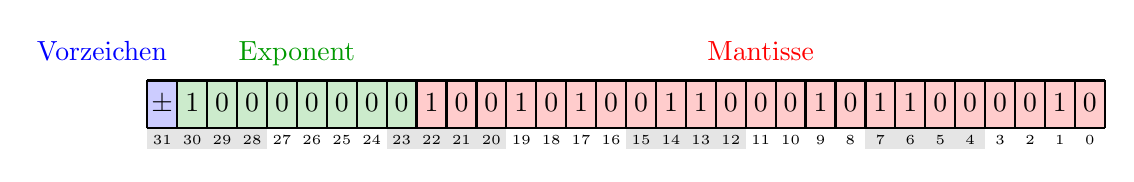
\begin{tikzpicture}[>=latex,thick,scale=0.38]

\definecolor{darkgreen}{rgb}{0,0.6,0}
\fill[color=blue!20]      (0,-0.8) rectangle (1,0.8);
\fill[color=darkgreen!20] (1,-0.8) rectangle (9,0.8);
\fill[color=red!20]       (9,-0.8) rectangle (32,0.8);

\node[color=blue]      at ( 1  ,0.8) [above left] {Vorzeichen\strut};
\node[color=darkgreen] at ( 5  ,0.8) [above] {Exponent\strut};
\node[color=red]       at (20.5,0.8) [above] {Mantisse\strut};

\fill[color=gray!20] ( 0,-0.8) rectangle ( 4,-1.5);
\fill[color=gray!20] ( 8,-0.8) rectangle (12,-1.5);
\fill[color=gray!20] (16,-0.8) rectangle (20,-1.5);
\fill[color=gray!20] (24,-0.8) rectangle (28,-1.5);

\foreach \k in {0,...,31}{
	\node at ({31.5-\k},{-1.2}) {\tiny \k};
}

\draw (0,0.8)--(32,0.8);
\foreach \x in {0,...,32}{
	\draw (\x,-0.8)--(\x,+0.8);
}
\draw (0,-0.8)--(32,-0.8);

\def\feld#1#2{
\node at ({#1+0.5},0) {$\mathstrut #2$};
}

\feld{0}{\pm}

\feld{1}{1}
\feld{2}{0}
\feld{3}{0}
\feld{4}{0}
\feld{5}{0}
\feld{6}{0}
\feld{7}{0}
\feld{8}{0}

\feld{9}{1}
\feld{10}{0}
\feld{11}{0}
\feld{12}{1}
\feld{13}{0}
\feld{14}{1}
\feld{15}{0}
\feld{16}{0}
\feld{17}{1}
\feld{18}{1}
\feld{19}{0}
\feld{20}{0}
\feld{21}{0}
\feld{22}{1}
\feld{23}{0}
\feld{24}{1}
\feld{25}{1}
\feld{26}{0}
\feld{27}{0}
\feld{28}{0}
\feld{29}{0}
\feld{30}{1}
\feld{31}{0}

\end{tikzpicture}
\end{center}
Die Ganzzahl $\texttt{10000000}_2=128_{10}$ im Exponentenfeld
muss um $127$ verringert werden um den Exponenten $1$ zu ergeben.

Die grösste und kleinste mit einem \texttt{float} darstellbare positive
Zahl ist somit
\begin{align*}
\texttt{1.11111111111111111111111}_2 \cdot 2^{\phantom{-}128}
&=
3.4028232_{10}\cdot 10^{\phantom{-}38}
\\
\texttt{1.00000000000000000000000}_2 \cdot 2^{-127}
&=
5.8774717_{10}\cdot 10^{-39}
\end{align*}
Den 24 binären Mantissenbits entsprechen gut 7 Dezimalstellen.

Genau genommen können noch etwas kleinere Zahlen dargestellt werden, wenn
man auf die Konvention verzichtet, dass vor dem Komma eine \texttt{1}
stehen muss.
Man nennt solche noch kleineren Zahlen {\em denomormalisiert}.
Da das Floatingpoint-Format immer auch eine implizite führende \texttt{1}
beinhaltet, braucht es zusätzliche Konventionen für denomarmalisierte Zahlen,
die die Abwesenheit der \texttt{1} signalisieren (Siehe auch den
Abschnitt Denormalisierung auf
Seite~\pageref{buch:zahlensysteme:denormalisierung}).

\begin{table}
\centering
\renewcommand\arraystretch{1.15}
\begin{tabular}{|l|>{$}l<{$}|>{$}l<{$}|>{$}l<{$}|}
\hline
&\texttt{float}&\texttt{double}&\texttt{long double}\\
\hline
kleinste darstellbare Zahl    &
	1.17549\cdot 10^{-38}&2.22507\cdot 10^{-308}&3.3621\cdot 10^{-4932}\\
grösste darstellbare Zahl     &
	3.40282\cdot10^{38} &1.79769\cdot10^{308} &1.18973\cdot10^{4932}\\
$\varepsilon$                 &
	1.19209\cdot 10^{-7}&2.22045\cdot 10^{-16}&1.0842\cdot 10^{-19}\\
kleinster Exponent            & -125&-1021&-16381\\
grösster Exponent             & 128&1024&16384\\
kleinste denormalisiert Zahl: &
	1.4013\cdot 10^{-45}&4.94066\cdot 10^{-324}&3.6452\cdot 10^{-4951}\\
\hline
\end{tabular}
\caption{Eigenschaften der Gleitkommatypen \texttt{float}, \texttt{double}
und \texttt{long double}.
Die Zeile $\varepsilon$ ist die Differenz zwischen 1 und der kleinsten
darstellbaren Zahl, die grösser ist als $1$.
Einzelne Exponentenwerte haben eine spezielle Bedeutung (siehe Text),
daher fallen die kleinstmöglichen Exponenten grösser aus als aufgrund
ihrer Bitlänge zu erwarten ist.
\label{buch:table:limits}}
\end{table}


\begin{table}
\centering
\begin{tabular}{|l|c|c|c|c|}
\hline
Typ&Bytes&Mantisse&Exponent&IEEE-754\\
\hline
\texttt{half},
\texttt{binary16}    &\phantom{0}2& \phantom{0}10 & \phantom{0}5     & * \\
\texttt{float},
\texttt{binary32}    &\phantom{0}4& \phantom{0}23 & \phantom{0}8     & * \\
\texttt{extended} 
                     &\phantom{0}5& \phantom{0}29 & 10               &   \\
\texttt{double},
\texttt{binary64}    &\phantom{0}8& \phantom{0}52 & 11               & * \\
\texttt{double extended},
\texttt{long double} &          10& \phantom{0}63 & 15               & * \\
\texttt{quad}
\texttt{binary128}   &          16& 112           & 15               & * \\
\texttt{binary256}   &          32& 236           & 19               & * \\
\hline
\end{tabular}
\caption{Übliche Gleitkommatypen mit Länge der Mantisse und des Exponenten.
Die meisten Compiler implementieren nur \texttt{float} und \texttt{double},
manchmal auch noch \texttt{long double}.
Die im Standard IEEE 754-2008 definierten Typen sind in der letzten Spalte
mit einen $*$ versehen.
\label{buch:table:ieee754}}
\end{table}

\subsubsection{Gebräuchliche Formate}
Der 1985 verabschiedete Standard IEEE~754 beschreibt die heute gebräuchlichen
Implementation von Gleitkommatypen abschliessend.
Damit ist gewährleistet, dass numerische Rechnungen auf verschiedenen
Prozessoren reproduzierbare Resultate geben.

Die C++-Standardbibliothek bietet im \texttt{<limits>} Header die Möglichkeit, 
Informationen über die Datentypen zu erhalten.
In Tabelle~\ref{buch:table:limits} sind die Eigenschaften der
gebräuchlichsten Typen zusammengestellt.
Allerdings offenbart sich hier auch ein Problem dieser Implementation
von \texttt{<limits>}.
Wie wir weiter unten sehen werden, definiert der IEEE 754 Standard
Werte für $\pm\infty$, die kleiner sind als die angegebenen
maximalen Werte.

Aktuelle Compiler unterstützen typischerweise die Gleitkomma-Typen
\texttt{float}, \texttt{double} und \texttt{long double}.
Bei Mikrokontrollern, wo Berechnungen mit der hohen Präzision
eines \texttt{double} nur schon wegen des Platzedarfs der Werte
und des Zeitbedarfs für die Operationen kaum sinnvoll sind, ist oft
nur der \texttt{float}-Typ implementiert.
Der GNU-Compiler für die 8-bit AVR-Prozessorfamilie stellt behandelt
zum Beispiel \texttt{double} genau gleich wie \texttt{float}.
Graphikkarten unterstützen oft noch einen halben Gleitkommatyp
\texttt{binary16}, dessen Genauigkeit für die Darstellung von 3D-Objekten
ausreichend ist.

\subsubsection{Rundung}
Der IEEE 754 Standard schreibt auch vor, wie Resultate gerundet werden
müssen.
\index{Rundungs-Regel}
Bei vielen Operationen entstehen Resultate, die einen längeren 
Nachkommateil haben als in das gegeben Gleitkommaformat passt,
das Resultat muss gerundet werden.
Der Standard kennt fünf verschiedene Rundungsverfahren und empfiehlt,
dass die Funktionen wie Wurzeln, Exponentialfunktionen,
trigonometrische Funktionen und viele weitere so implementiert werden 
müssen, dass das Resultat korrekt gerundet ist.
Damit ist gemeint, dass das Resultat entsteht, in dem auf das
mathematisch exakte Resultat die gewählte Rundungs-Regel angewendet
wird.

Der Standard bezweckt mit diesen Regeln, dass man sich im Rahmen der
Rundungsgenauigkeit auch auf die letzte Stelle eines Gleitkommawertes
verlassen kann.
Dies ist keinen Selbstverständlichkeit.
Gleitkomma-Implementationen von GPUs beispielsweise erfüllen diese
\index{GPU}
Bedingung oft nicht und garantieren in ihren Spezifikation manchmal
nur korrekte Resultate mit Ausnahme der letzten 1-2 bits.

\subsubsection{Die Null}
Die Gleitkomma-Darstellung definiert, dass die Mantisse ein implizites
führends \texttt{1}-bit hat. 
In diesem Format lässt sich die Null aber nicht darstellen, es ist
also eine separate Definition nötig:
\begin{itemize}
\item Alle Exponentenbits $=\texttt{0}$.
\item Alle Mantissenbits $=\texttt{0}$.
\item Vorzeichen $\texttt{0}$ oder $\texttt{1}$ erlaubt die Unterscheidung
zwischen $+0$ und $-0$.
\end{itemize}
Dies ist ein Spezialfall einer denormalisierten Zahl (siehe auch
Abschnitt Denormalisierung weiter unten auf
Seite~\pageref{buch:zahlensysteme:denormalisierung}).

\subsubsection{Unendlich grosse Werte}
Im Laufe einer numerischen Berechnung kann es vorkommen, dass die Resultate
so gross werden, dass sie nicht mehr im gegebenen Gleitkommatyp gespeichert
werden können.
Der Standard verlangt, dass diese Situation durch einen speziellen Wert
für unendlich grosse Zahlen wiedergegeben werden kann, der wie
folgt definiert ist:
\begin{itemize}
\item Alle Exponenten-Bits $= \texttt{1}$
\item Alle Mantissenbits $=\texttt{0}$
\item Vorzeichenbit \texttt{0} oder \texttt{1} um zwischen
$+\infty$ und $-\infty$ unterscheiden zu können.
\end{itemize}
Dies bedeutet, dass der grösste nutzbare Exponent des $\texttt{float}$-Typs
nur noch $127$ ist.

\subsubsection{Denormalisierung
\label{buch:zahlensysteme:denormalisierung}}
\index{denormalisierte Zahl}%
Die Mantisse einer Gleitkommazahl beginnt immer mit einer 1, die aber
nicht gespeichert wird.
Wird eine Zahl kleiner als mit dem zur Verfügung stehenden Exponenten-Bereich
darstellbar, kann sie nicht mehr in diesem Format gespeichert werden.
Um solche Zahlen darzustellen, wurde vom Standard einem Exponenten aus
lauter \texttt{0} eine besondere Bedeutung gegeben.
Für den Typ \texttt{float} entspricht er nicht mehr dem Exponenten $-127$
sondern $-126$ und das implizite führend Bit der Mantisse ist jetzt 0.
Mit diesen sogenannten denormalisierten Zahlen lassen sich noch kleinere
Wert darstellen, die aber nicht mehr so präzis sind, weil sie weniger
signifikante Stellen aufweisen.

\subsubsection{Vor- und Nachteile}
\begin{itemize}
\item[$\oplus$]
Wir eine beliebige reelle Zahl als Gleitkommazahl abgespeichert, muss
sie um maximal um den halben Wert des letzten Mantissebits gerundet werden.
Der absolute Wert desselben hängt jedoch vom Exponenten ab.
Bei $l$ Mantissenbits ist er aber immer um den Faktor $2^l$ kleiner
als die Zahl selbst.
Es tritt ein konstanter {\em relativer} Fehler auf.
\item[$\oplus$] Dank des grossen Wertebereiches sind Über- und Unterlauf
unwahrscheinlich.
\item[$\ominus$]
Gleitkommazahlen brauchen mehr Speicherplatz.
Der kleinste Gleitkommatyp \texttt{float} ist mit 32 bit bereits so gross wie
der gebräuchlichste Ganzzahltyp \texttt{long}.
\item[$\ominus$] Geschwindigkeit: sofern keine Hardware-Beschleunigung
zur Verfügung steht sind Gleitkomma-Operationen deutlich langsamer
als Operationen mit Festkomma-Zahlen.
\item[$\ominus$]
In einer Multi-Core CPU hat nicht unbedingt jeder Kern eine Gleitkomma-Einheit.
Gleitkommaoperationen in verschiedenen Threads können sich also gegenseitig
behindern.
\end{itemize}

%
% Hochpräzisionsbibliotheken
%
\subsection{Hochpräzisionsbibliotheken
\label{buch:subsection:mp}}
Die Diskussion numerischer Effekte in
Abschnitt~\label{buch:section:numerische-effekte} zeigen, dass es nötig sein
kann, Berechnungen mit sehr viel höherer Präzision durchzuführen, um die
Genauigkeit des Schlussresultats garantieren zu können.
Weder die Gleitkomma-Datentypen noch die Arithmetik-Prozessoren der
CPUs unterstützen aber beliebig grosse Gleitkommazahlen.
Es müssen daher Bibliotheken verwendet werden, die solche Datentypen
und die arithmetischen Operationen nachbilden.

Als Beispiel soll die Exponentialfunktion $e^{-100}$ mit
Hilfe der Taylor-Reihe
\[
e^x
=
1 + x + \frac{x^2}{2!} + \frac{x^3}{3!} + \frac{x^4}{4!} + \dots
=
\sum_{k=0}^\infty \frac{x^k}{k!}
\]
berechnet werden.
Die Berechnung der einzelnen Terme kann dank der Formel
\begin{equation}
\frac{x^k}{k!}
=
\frac{x^k}{1\cdot 2\cdot 3 \cdot \ldots \cdot (k-1)\cdot k}
=
\frac{x}{1}
\cdot
\frac{x}{2}
\cdot
\frac{x}{3}
\cdot\dots\cdot
\frac{x}{k-1}
\cdot
\frac{x}{k}
\label{buch:eulerreihe:faktor}
\end{equation}
iterativ mit einer einfachen Multiplikation mit dem ``nächsten'' 
Faktor $x/k$ erfolgen.

In Abschnitt~\ref{buch:subsection:verschiebung} wird gezeigt, dass
für negative Argument $x$ die Berechnung wegen Verschmierung mit sehr
viel grösserer Genauigkeit durchgeführt werden muss, wenn das Resultat
exakt sein soll.
Das Problem kann behoben werden, wenn man für negatives $x$
die Formel $e^x = 1/e^{-x}$ ausnutzt und die die Taylor-Reihe
auf das Argument $-x$ anwendet, wo die Schwierigkeit nicht auftritt.

In diesem Beispiel wird dieses Problem illustriert, indem die gleiche
Berechnung mit verschiedener Genauigkeit mit einer Hochpräzisionsbibliothek
durchgeführt wird.
Dazu wird das Treiberprogramm von Listing~\ref{numerik:listing:main}
verwendet.
\begin{lstlisting}[float,style=C,caption={Treiber-Programm zur Berechnung von $e^x$ mit verschiedenen Hochpräzisionsbibliotheken.},label={numerik:listing:main}]
int     main(int argc, char *argv[]) {
        int     bits = 32;
        while (bits <= 512) {
                experiment(bits);
                bits <<= 1;
        }

        return EXIT_SUCCESS;
}
\end{lstlisting}
Die Implementation der Funktion \texttt{experiment(double x)} mit 
verschiedenen Hochpräzisionsbibliotheken wird weiter unten beschrieben.
Man erwartet, dass bei ausreichend grosser Präzision ein ausreichend
genaues Resultat erhalten werden kann.

\subsubsection{GNU GMP}
Die freie GNU GMP Bibliothek erschien 1991 und kann auf \url{http://gmplib.org}
gefunden werden.
Die Implementation ist nicht zu IEEE 754 konform und es ist nicht garantiert,
dass verschiedene Maschinen identische Resultate mit dem gleichen Code
erhalten.
Daher wird empfohlen, für neue Projek die MPFR Bibliothek (siehe nächsten
Abschnitt) zu verwenden.
\begin{lstlisting}[float,style=C,caption={C-Programm zur Berechnung von $e^x$ mit Hilfe der Taylor-Reihe, implementiert mit GMP},label={numerik:listing:gmp}]
#include <gmp.h>
#include <stdio.h>
#include <stdlib.h>
#include <math.h>

double  gmpexp(double x) {
        mpf_t   X, P, S;
        /* Variablen initialisieren */
        mpf_init(X);
        mpf_init(P);
        mpf_init(S);
        mpf_set_d(X, x);
        mpf_set_d(P, 1.);
        mpf_set_d(S, 1.);

        /* Hilfsvariablen fuer Zwischenresultate */
        mpf_t   R, Q;
        mpf_init(R);
        mpf_init(Q);

        for (int i = 1; i < 1000; i++) {
                /* P = P * X / i */
                mpf_mul(Q, P, X);
                mpf_div_ui(R, Q, i);
                mpf_set(P, R);
                /* S = S + P */
                mpf_add(Q, S, P);
                mpf_set(S, Q);
        }

        double  result = mpf_get_d(S);

        mpf_clear(X);
        mpf_clear(P);
        mpf_clear(S);
        mpf_clear(R);
        mpf_clear(Q);

        return result;
}

void    experiment(int bits) {
        /* Setze Mindestgenauigkeit der Variablen */
        mpf_set_default_prec(bits);
        double  x = -100;
        double  y = gmpexp(x);
        double  z = exp(x);

        printf("bits:         %d\n", bits);
        printf("GMP:          %.20g\n", y);
        printf("Prozessor:    %.20g\n", z);
        printf("Fehler:       %.20g\n\n", y - z);
}
\end{lstlisting}

Der Code in Listing~\ref{numerik:listing:gmp} zeigt die Berechnung der
Taylor-Reihe mit Hilfe von GNU GMP.
In Zeile 44 in der Funktion \texttt{void experiment(int bits)} wird die
minimale Genauigkeit, mit der die Bibliothek rechnen soll.
Die Aufrufe von \verb+mpf_init(mpf_t op)+ in der Funktion
\texttt{double gmpexp(double x)} initialisieren die Variablen
mit mindstens dieser Genauigkeit.
Welche Genauigkeit genau gewählt wird hängt von der Wortlänge der
verwendeten Maschine ab.

In den Zeilen 21--29 wird die Taylor-Reihe summiert.
In der Variable \texttt{P} ist der Wert des aktuellen Summanden
gespeichert.
Der nächste Summand kann daraus gemäss \eqref{buch:eulerreihe:faktor}
mittels $\texttt{P}\cdot x/i$
berechnet werden, wobei $i$ der Wert der Zählervariablen ist,
mit der die Summanden indiziert werden.
In Zeile~31 wird die Summe wieder in einen \texttt{double}-Wert
mit Maschinenpräzision umgewandelt.


\begin{table}
\centering
\begin{tabular}{|>{$}r<{$}|>{$}r<{$}|>{$}r<{$}|>{$}r<{$}|}
\hline
\text{Bits} & \text{GNU GMP} & \texttt{double} &\text{Fehler} \\
\hline
 32 &
-2.378447678\cdot 10^{\phantom{-}19} &
 3.720075976\cdot 10^{-44}           &
-2.378447678\cdot 10^{\phantom{-}19}
\\
 64 &
-2.378447678\cdot 10^{\phantom{-}19} &
 3.720075976\cdot 10^{-44}           &
-2.378447678\cdot 10^{\phantom{-}19} 
\\
 128 &
 1.384432347\cdot 10^{\phantom{-0}1} &
 3.720075976\cdot 10^{-44}           &
 1.384432347\cdot 10^{\phantom{-0}1}
\\
 256 &
-1.339761431\cdot 10^{-39} &
 3.720075976\cdot 10^{-44} &
-1.339798632\cdot 10^{-39}
\\
 512 &
 3.720075976\cdot 10^{-44} &
 3.720075976\cdot 10^{-44} &
-4.978412222\cdot 10^{-60}
\\
\hline
\end{tabular}
\caption{Tabelle der Resultate der Berechnung von $e^{-100}$ mit Hilfe
der Taylor-Reihe der Exponentialfunktion unter Verwendung des Programms
von Listing~\ref{numerik:listing:gmp} mit verschiedenen Bitlängen.
\label{numerik:expresultate:gmp}}
\end{table}

Die Resultate der Berechnung sind in Tabelle~\ref{numerik:expresultate:gmp}
zusammengestellt.
Die Spalte \texttt{double} enthält die mit der Formel $e^x = 1/e^{-x}$ mit
Maschinengenauigkeit erhaltenen Werte mit Maschinengenauigkeit.
Zunächst fällt auf, dass der Fehler der Berechnung mit 32 bit und mit 64 bit
gleich gross ist.
Dies rührt daher, dass die Bibliothek für die 32 bit Rechnung die gleiche
Genauigkeit verwendet wie bei 64 bit.
Selbst die Präzision von 256 bit reicht nicht aus, um $e^{-100}$ zu
berechnen.
Erst im letzten Resultat stimmt das Resultat mit 16 signifikanten Stellen.
Eine genauere Untersuchung zeigt, dass die volle Genauigkeit bei
384 bits erreicht wird.

\subsubsection{GNU Multiple Precision Floating-Point Reliable Library}
Die GNU Multiple Precision Floating-Point Reliable Library versucht,
die Defizite der GMP zu kompensieren.
Das nur wenig abweichende Listing~\ref{numerik:listing:mpfr} zeigt
die Implementation.

Mit der Funktion \verb+mpfr_set_default_prec(int bits)+ in Zeile~44
wird nicht die minimale sondern die exakte Anzahl Bits festgelegt,
mit der gerechnet werden soll.
Bei jeder Operation, bei der gerundet werden muss, kann spezifiziert
werden, in welche Richtung die Rundung vorgenommen werden soll, dies
ist die Bedeutung der Konstaten \verb+MPFR_RNDN+.
Schliesslich ist die Implementation konform mit dem IEEE 754 Standard,
so dass bei Verwendung dieser Bibliothek garantiert ist, dass die
Resultate nicht von der Plattform abhängen.

\begin{lstlisting}[float,style=C,caption={C-Programm zur Berechnung von $e^x$ mit Hilfe der Taylor-Reihe, implementiert mit MPFR},label={numerik:listing:mpfr}]
#include <mpfr.h>
#include <stdio.h>
#include <stdlib.h>
#include <math.h>

double  mpfrexp(double x) {
        mpfr_t  X, P, S;
        /* Variablen initialisieren */
        mpfr_init(X);
        mpfr_init(P);
        mpfr_init(S);
        mpfr_set_d(X, x, MPFR_RNDN);
        mpfr_set_d(P, 1., MPFR_RNDN);
        mpfr_set_d(S, 1., MPFR_RNDN);

        /* Hilfsvariablen fuer Zwischenresultate */
        mpfr_t  R, Q;
        mpfr_init(R);
        mpfr_init(Q);

        for (int i = 1; i < 1000; i++) {
                /* P = P * X / i */
                mpfr_mul(Q, P, X, MPFR_RNDN);
                mpfr_div_ui(R, Q, i, MPFR_RNDN);
                mpfr_set(P, R, MPFR_RNDN);
                /* S = S + P */
                mpfr_add(Q, S, R, MPFR_RNDN);
                mpfr_set(S, Q, MPFR_RNDN);
        }

        double  result = mpfr_get_d(S, MPFR_RNDN);

        mpfr_clear(X);
        mpfr_clear(P);
        mpfr_clear(S);
        mpfr_clear(R);
        mpfr_clear(Q);

        return result;
}

void    experiment(int bits) {
        /* Setze exakte Genauigkeit der Variablen */
        mpfr_set_default_prec(bits);
        double  x = -100;
        double  y = mpfrexp(x);
        double  z = exp(x);

        printf("bits:         %d\n", bits);
        printf("GMP:          %.20g\n", y);
        printf("Prozessor:    %.20g\n", z);
        printf("Fehler:       %.20g\n\n", y - z);
}
\end{lstlisting}


\begin{table}
\centering
\begin{tabular}{|>{$}r<{$}|>{$}r<{$}|>{$}r<{$}|>{$}r<{$}|}
\hline
\text{Bits} & \text{GNU MPFR} & \texttt{double} &\text{Fehler} \\
\hline
32 &
 4.040280437\cdot 10^{\phantom{-}32} &
 3.720075976\cdot 10^{-44} &
 4.040280437\cdot 10^{\phantom{-}32}
\\
64 &
-1.797196708\cdot 10^{\phantom{-}23} &
 3.720075976\cdot 10^{-44}           &
-1.797196708\cdot 10^{\phantom{-}23} 
\\
128 &
 3.777954147\cdot 10^{\phantom{-0}3} &
 3.720075976\cdot 10^{-44} &
 3.777954147\cdot 10^{\phantom{-0}3}
\\
256 &
-5.943812579\cdot 10^{-39} &
 3.720075976\cdot 10^{-44} &
-5.943849780\cdot 10^{-39}
\\
328 &
 3.720075976\cdot 10^{-44} &
 3.720075976\cdot 10^{-44} &
 3.196140646\cdot 10^{-57}
\\
329 &
 3.720075976\cdot 10^{-44} &
 3.720075976\cdot 10^{-44} &
-1.941580766\cdot 10^{-58}
\\
330 &
 3.720075976\cdot 10^{-44} &
 3.720075976\cdot 10^{-44} &
 5.326901077\cdot 10^{-58}
\\
331 &
 3.720075976\cdot 10^{-44} &
 3.720075976\cdot 10^{-44} &
 4.132082144\cdot 10^{-58}
\\
332 &
 3.720075976\cdot 10^{-44} &
 3.720075976\cdot 10^{-44} &
 7.467618333\cdot 10^{-59}
\\
333 &
 3.720075976\cdot 10^{-44} &
 3.720075976\cdot 10^{-44} &
-8.463300777\cdot 10^{-59}
\\
334 &
 3.720075976\cdot 10^{-44} &
 3.720075976\cdot 10^{-44} &
-9.956824444\cdot 10^{-60}
\\
512 &
 3.720075976\cdot 10^{-44} &
 3.720075976\cdot 10^{-44} &
 0\phantom{.000000000\cdot 10^{-00}}
\\
\hline
\end{tabular}
\caption{Tabelle der Resultate der Berechnung von $e^{-100}$ mit Hilfe
der Taylor-Reihe der Exponentialfunktion unter Verwendung des Programms
von Listing~\ref{numerik:listing:mpfr} mit verschiedenen Bitlängen.
\label{numerik:expresultate:mpfr}}
\end{table}

In Tabelle~\ref{numerik:expresultate:mpfr} sind die Resultate
zusammengestellt.
Es fällt sofort auf, dass 32 bit und 64 bit verschiedene Resultate
geben.
Ab Bitlänge 328 ist in den gezeigten Stellen kein Unterschied mehr zwischen 
der Maschinenimplementation und der MPFR-Implementation erkennbar,
trotzdem verbleibt eine Abweichung, der in der letzten Spalte dargestellt
wird.
Sie zeigt auch, dass in der MPFR-Implementation jedes einzelne Bit
einen Unterschied macht.
Die MPFR-Bibliothek kann daher auch als Labor für Experimente über
die Abhängigkeit der Fehler von der Genauigkeit der Arithmetik dienen.

Die Programmierung mit diesen Bibliotheken ist wegen der
vielen Funktionsaufrufe eher etwas mühsam.
Moderne C++-Wrapper ermöglichen dank Operator-Überladung eine intuitivere
Notation.


%
% effekte.tex
%
% (c) 2020 Prof Dr Andreas Müller, Hochschule Rapperswil
%
\section{Numerische Effekte
\label{buch:section:numerische-effekte}}
\rhead{Numerische Effekte}

\subsection{Auslöschnung}

\subsection{Verschmierung}


%
% iteration.tex
%
% (c) 2020 Prof Dr Andreas Müller, Hochschule Rapperswil
%
\section{Iteration
\label{buch:section:iteration}}
\rhead{Iteration}
Die meisten numerischen Problemlösungen mit einem Computer nutzen deren
Fähigkeit aus, dieselbe Rechnung immer wieder zu wiederholen, bis zum
Beispiel die gewünschte Genauigkeit erziehlt ist.
Es lohnt sich daher ganz unabhängig irgendwelchen Einschränkungen 
der Computer-Hardware zu überlegen, was passiert, wenn man eine
Funktion $f\colon \mathbb R\to\mathbb R$ immer wieder auf ihren eigenen
Output anwendet, wie das zum Beispiel der Code in einer Schleife
bei jedem Durchlauf macht.

In diesem Abschnitt ist also
\[
f\colon \mathbb{R}\to\mathbb{R} : x\mapsto f(x)
\]
eine differenzierbare Funktion.
Mit einem gegebenen Startwert $x_0\in\mathbb R$ lässt sich durch
wiederholte Anwendung von $f$ die Folge
\[
x_0,\; x_1 = f(x_0),\; x_2 = f(x_1),\; x_3 = f(x_2),\; x_4 = f(x_3),\dots
\]
konstruieren.

Ist der Punkt $x^*$ ein {\em Fixpunkt} der Funktion $f(x)$, ist also
$f(x^*)=x^*$,
\index{Fixpunkt}%
dann ist die mit $x_0=x^*$ gebildete Iterationsfolge konstant.
Es stellt sich damit automatisch die Frage, was mit einem von $x^*$
abweichenden Startwert passiert. Entfernen sich die Werte $x_k$ von $x^*$
oder konvergiert die Folge am Ende gegen $x^*$?

%
% Beispiele
%
\subsection{Beispiele}
Wir illustrieren die verschiedenen Situation, die beim Iterieren der
Funktion $f$ auftreten können an einigen Beispielen.

\begin{beispiel}
\label{section:beispiel:sqrtiteration}
Wir betrachten die Funktion 
\[
f\colon \mathbb{R}\to\mathbb{R} : x\mapsto \sqrt{x+2}
\]
Die Iterationsfolge ausgehend vom Startwert $x_0=0$ ist in
Tabelle~\ref{buch:table:sqrtiteration} dargestellt.

\begin{table}
\centering
\renewcommand\arraystretch{1.15}
%
% sqrtiteration.tex -- generated by sqrtiteration.m
%
% (c) 2020 Prof Dr Andreas Müller Hochschule Rapperswil
%
\begin{tabular}{|>{$}r<{$}|>{$}r<{$}|>{$}r<{$}|>{$}r<{$}|}
\hline
   k & x_k                           & \delta_k = 2-x_k     & \delta_{k-1} / \delta_{k} \\
\hline
  0 &             0.0000000000000000 &   2.0000000000000000 &        \\
  2 &             1.4142135623730951 &   0.5857864376269049 & 3.4142 \\
  3 & \underline{1.8}477590650225735 &   0.1522409349774265 & 3.8478 \\
  4 & \underline{1.9}615705608064609 &   0.0384294391935391 & 3.9616 \\
  5 & \underline{1.99}03694533443939 &   0.0096305466556061 & 3.9904 \\
  6 & \underline{1.997}5909124103448 &   0.0024090875896552 & 3.9976 \\
  7 & \underline{1.999}3976373924085 &   0.0006023626075915 & 3.9994 \\
  8 & \underline{1.9998}494036782890 &   0.0001505963217110 & 3.9998 \\
  9 & \underline{1.9999}623505652022 &   0.0000376494347978 & 4.0000 \\
 10 & \underline{1.99999}05876191524 &   0.0000094123808476 & 4.0000 \\
 11 & \underline{1.999997}6469034038 &   0.0000023530965962 & 4.0000 \\
 12 & \underline{1.999999}4117257645 &   0.0000005882742355 & 4.0000 \\
 13 & \underline{1.9999998}529314358 &   0.0000001470685642 & 4.0000 \\
 14 & \underline{1.9999999}632328584 &   0.0000000367671416 & 4.0000 \\
 15 & \underline{1.99999999}08082147 &   0.0000000091917853 & 4.0000 \\
 16 & \underline{1.999999997}7020537 &   0.0000000022979463 & 4.0000 \\
 17 & \underline{1.999999999}4255133 &   0.0000000005744867 & 4.0000 \\
 18 & \underline{1.9999999998}563782 &   0.0000000001436218 & 4.0000 \\
 19 & \underline{1.9999999999}640945 &   0.0000000000359055 & 4.0000 \\
 20 & \underline{1.99999999999}10236 &   0.0000000000089764 & 4.0000 \\
 21 & \underline{1.999999999997}7558 &   0.0000000000022442 & 3.9998 \\
 22 & \underline{1.999999999999}4389 &   0.0000000000005611 & 3.9996 \\
 23 & \underline{1.9999999999998}597 &   0.0000000000001403 & 3.9984 \\
 24 & \underline{1.9999999999999}649 &   0.0000000000000351 & 4.0000 \\
 25 & \underline{1.99999999999999}11 &   0.0000000000000089 & 3.9500 \\
 26 & \underline{1.999999999999997}8 &   0.0000000000000022 & 4.0000 \\
 27 & \underline{1.999999999999999}3 &   0.0000000000000007 & 3.3333 \\
 28 & \underline{1.9999999999999998} &   0.0000000000000002 & 3.0000 \\
 29 & \underline{2.0000000000000000} &   0.0000000000000000 &        \\
 30 & \underline{2.0000000000000000} &   0.0000000000000000 &        \\
\hline
\end{tabular}

\caption{Iterationsfolge für die Funktion $f(x)=\sqrt{x+2}$ ausgehend
vom Startwert $x_0=0$.
\label{buch:table:sqrtiteration}}
\end{table}

Die Werte konvergieren offenbar gegen den Wert $2$, 
In der dritten Spalte steht die Abweichung $\delta_k$ des $k$-ten Folgengliedes
vom Grenzwert $2$.
Mit jeder Iteration wird der Fehler um den Faktor 4 kleiner, wie die
vierte Spalte zeigt, in der Quotient aufeinanderfolgender Fehler
berechnet ist.

Dieses Verhalten des Fehlers kann man auch analytisch verstehen.
Nehmen wir an, dass $x_n = 2 + \delta_n$ und versuchen wir 
$x_{n+1}$ zu berechnen.
Indem wir die Funktion $f(x)$ im Punkt $x=2$ mit Hilfe der Ableitung
linear approximieren, erhalten wir wegen
\[
f'(x) = \frac{1}{2\sqrt{x+2}}
\]
den Wert
\[
x_{n+1} = f(x_n) = f(2 + \delta_n)
\simeq
f(2) + f'(2)\cdot \delta_n
2 + \underbrace{\frac14\cdot \delta_n}_{\displaystyle\simeq\delta_{n+1}}
\]
für $x_{n+1}$.
Der Fehler von $x_{n+1}$ ist also $\delta_{n+1}\simeq\frac14\delta_n$.
In jedem Iterationsschritt gewinnen wir daher etwa 2 bit Genauigkeit.
Für die 52 bit Mantisse des \texttt{double} Typs brauchen wir also
etwa 26 Iterationen.
\end{beispiel}

\begin{beispiel}
\label{buch:beispiel:logistisch3}
Wir betrachten die Funktion
\[
f(x) = 3x(1-x).
\]
Sie hat zwei Fixpunkte, die man durch Lösen der quadratischen
Gleichung
\[
f(x^*)=x^*
\quad\Rightarrow\quad
x^*=-3x^{*2}+3x^*
\quad\Rightarrow\quad
3x^{*2}-2x^*=3x^*(x^*-{\textstyle\frac23})=0
\quad\Rightarrow\quad
x^*=
\begin{cases}
0      &\\
\frac23&
\end{cases}
\]
findet.

Für einen Startwert $x_0$ nahe des Fixpunktes $x^*=0$ gilt
\[
f(\delta)
=
3\delta(1-\delta)
=
3\delta - 3\delta^2.
\]
Für kleine Werte von $\delta$ kann man den quadratischen Term vernachlässigen
und sieht, dass der Fehler durch die Iteration verdreifacht wird.
Konvergenz zu diesem Fixpunkt ist also nicht möglich.

Für den Fixpunkt $x^* = \frac23$ finden wir
\begin{equation}
f({\textstyle\frac23}+\delta)
=
3({\textstyle\frac23}+\delta)({\textstyle\frac13}-\delta)
=
\frac{(2+3\delta)(1-3\delta)}3
=
\frac{2-3\delta+9\delta^2}{3}
=
\frac23 - \delta  + 9\delta^2
\label{buch:equation:logistic3error}
\end{equation}
Der Fehler $\delta$ wird zu $ -\delta(1-9\delta) $, er ändert also sein
Vorzeichen.
Ist $\delta>0$ wird der Fehlerbetrag wird nur um den Faktor $1-9\delta < 1$
reduziert.
Ist aber $\delta <0$, dann ist $1-9\delta>0$, der Fehlerbetrag wird wieder
vergrössert.

Sei jetzt $\delta>0$, wir wollen den Fehler nach zwei Iterationsschritten
berechnen.
Nach dem ersten ist der Fehler $\delta(1-9\delta)$, nach dem zweiten
\[
\delta(1-9\delta)(1-\delta(1-9\delta))
=
\delta(1-18\delta + 162\delta^2-729\delta^3).
\]
Für kleines $\delta$ können die Terme höhrer als erster Ordnung
vernachlässigt werden und man kann schliessen, dass der Fehler nach
zwei Iterationen tatsächlich um den Faktor $(1-18\delta)$ kleiner
geworden ist.

\begin{figure}
\centering
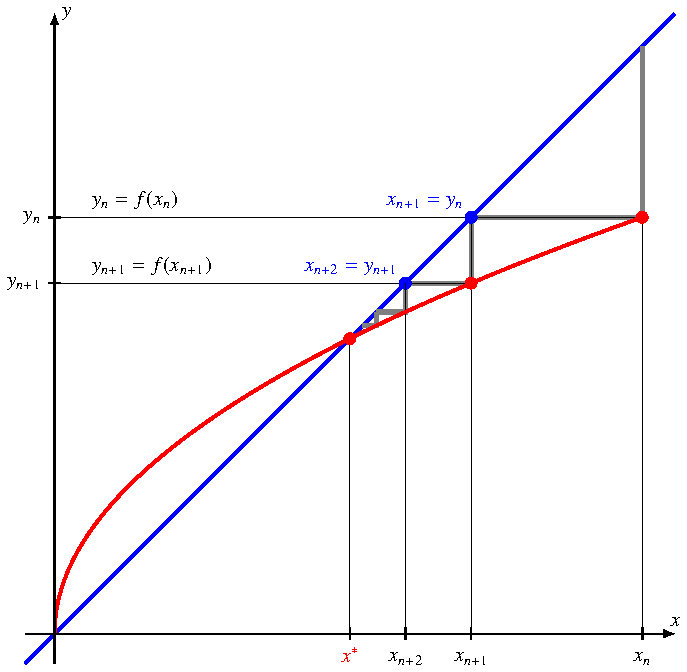
\includegraphics{chapters/10-arithmetik/figures/iteration.pdf}
\caption{Ein Fixpunkt $x^*$ der Funktion $f(x)$ manifestiert sich als
Schnittpunkt des Graphen $y=f(x)$ mit der $45^\circ$-Geraden.
Die Iterationsfolge ausgehend von einem Startwert $x_0$ wird als
Treppenkurve zwischen dem Graphen von $f$ und der $45^\circ$-Geraden
sichtbar.
\label{buch:figure:iterationprinzip}}
\end{figure}

Wir möchten wissen, wieviele Iterationsschritte nötig sind, um eine
bestimmte Genauigkeit zu erreichen.
Wir möchten also den Fehler $\delta_{2n}$ vorgeben und das zugehörige
$n$ bestimmen.
Wie wir soeben berechnet haben, nimmt der Betrag des Fehlers zwischen
den Schritten $k$ und $k+2$ gemäss
\[
\delta_{k+2} = \delta_{k} (1-18\delta_k)
\]
um den Faktor $(1-18\delta_k)$ ab.
Es ist übersichtlicher, mit dem Logarithmus des Fehlers zu rechnen.
Dieser verändert sich gemäss
\[
\log \delta_{k+2}
=
\log \delta_{k} + \log(1-18\delta_k)
\simeq
\log\delta_k - 18\delta_k,
\]
wobei wir für den zweiten Term die lineare Approximation aus der
Taylorreihe
\[
\log (1+x) = x - \frac{x^2}2 + \frac{x^3}3 -\dots
\]
von 
$\log x $ an der Stelle $x=1$ verwendet haben.
Zwischen $\delta_0$ und $\delta_{2n}$ bedeutet dies
\[
\log\delta_{2n}
=
\log\delta_0
-18
\sum_{k=0}^{n-1} \delta_{2k}
\qquad\Rightarrow\qquad
\frac1{18}
\log\frac{\delta_0}{\delta_{2n}}
=
\sum_{k=0}^{n-1}\delta_{2k}.
\]
Da der Fehler immer kleiner wir, kann man für eine erste grobe Abschätzung
der Summe auf der rechten Seite die grössten und kleinsten Terme
verwenden, um die Summe nach und unten und oben durch
\[
n\delta_{2n-2}
\le
\sum_{k=0}^{n-1}\delta_{2k}
\le
n\delta_0.
\]
abzuschätzen
Einsetzen ergibt
\[
n\delta_{2n-2}
\le
\frac{1}{18}
\log\frac{\delta_{0}}{\delta_{2n}}
\le
n\delta_0
\quad\Rightarrow\quad
\frac{1}{18\delta_0}
\log\frac{\delta_{0}}{\delta_{2n}}
\le
n
\le
\frac{1}{18\delta_{2n-2}}
\log\frac{\delta_{0}}{\delta_{2n}}
<
\frac{1}{18\delta_{2n}}
\log\frac{\delta_{0}}{\delta_{2n}}.
\]
Eine Verbesserung um zwei Stellen von $\delta_0=0.01$ auf $\delta_{2n}=0.0001$
braucht also zwischen $25$ und $2558$ Iterationen.
\end{beispiel}

%
% Graphische Analyse
%
\subsection{Graphische Analyse
\label{buch:section:graphischeanalyse}}
Ein Fixpunkt der Funktion $f(x)$ manifestiert sich in einem 
Schnittpunkte des Graphen von $f$ mit der $45^\circ$-Geraden
$y=x$ wie in Abbildung~\ref{buch:figure:iterationprinzip}.
Die Iterationsfolge $x_n$ kann graphisch wie folgt dargestellt
werden.
Ausgehend vom Wert $x_n$ auf der $x$-Achse folgt man der Vertikalen,
bis man auf den Graphen der Funktion $f$ trifft, dies liefert den
Wert $y_n=f(x_n)$.
Dieser soll jetzt als neuer $x$-Wert verwendet werden.
Dazu folgt man der Horizontalen bis zur $45^\circ$-Geraden,
die $x$-Koordinate des Schnittpunktes ist $x_{n+1}$.
So entsteht Treppenlinie in Abbildung~\ref{buch:figure:iterationprinzip}.

%
% Konvergenzbedingung
%
\subsection{Konvergenzbedingung
\label{buch:subsection:konvergenzbedingung}}
%
% graphisch0.tex
%
% (c) 2020 Prof Dr Andreas Müller, Hochschule Rapperswil
%
\begin{figure}
\centering
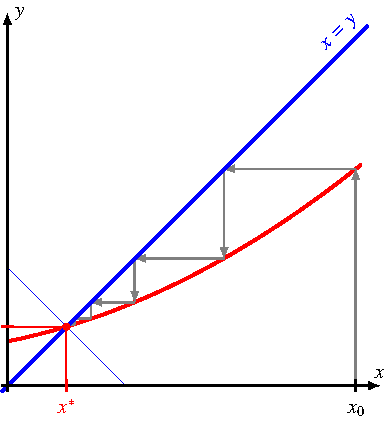
\includegraphics{chapters/10-arithmetik/figures/normal.pdf}
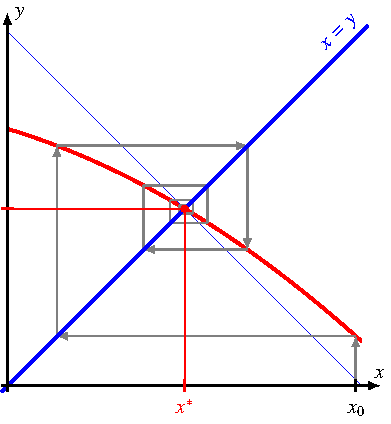
\includegraphics{chapters/10-arithmetik/figures/negativ.pdf}
\caption{Die Fixpunktiteration $x_{n+1}=f(x_n)$ konvergiert gegen
den Fixpunkt $x^*$ falls $|f'(x^*)|<1$ mit
mindestens linearer Konvergenzgeschwindigkeit.
\label{buch:figure:fixpunkt:normal}}
\end{figure}

%
% graphisch1.tex
%
% (c) 2020 Prof Dr Andreas Müller, Hochschule Rapperswil
%
\begin{figure}
\centering
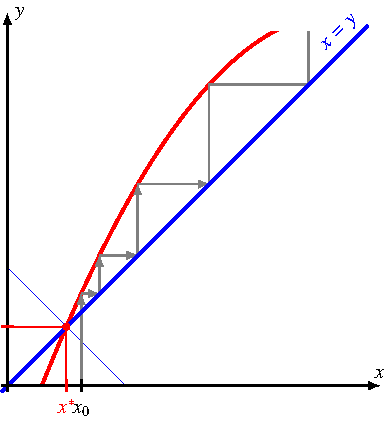
\includegraphics{chapters/10-arithmetik/figures/divergent.pdf}
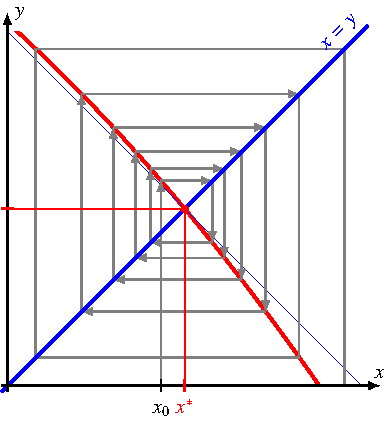
\includegraphics{chapters/10-arithmetik/figures/negdiv.pdf}
\caption{Die Fixpunktiteration $x_{n+1}=f(x_n)$ mit Fixpunkt $x^*$
divergiert für $|f'(x^*)|>1$.
\label{buch:figure:fixpunkt:divergent}}
\end{figure}

Aus der graphischen Analyse von Abschnitt~\ref{buch:section:graphischeanalyse}
kann man jetzt leicht Kriterien ableiten, wann die Iterationsfolge
konvergent ist.
Die Situation in Abbildung~\ref{buch:figure:iterationprinzip}
tritt zum Beispiel immer ein, wenn in einer Umgebung von $x^*$ 
der Graph der Funktion $f$ zwischen der horizontalen und der 
$45^\circ$-Geraden verläuft, oder anders ausgedrückt, wenn
\[
\begin{aligned}
x^* &< f(x) < x &&& &\text{für $x>x^*$ und} \\
x^* &> f(x) < x &&& &\text{für $x<x^*$}
\end{aligned}
\]
gilt.

Ist dagegen der Graph von $f$ in einer Umgebung von $x^*$ steiler als
die $45^\circ$-Gerade, dann gilt 
\begin{equation}
f(x) \;\begin{cases}
> x&\qquad\text{für $ x>x^*$}\\
< x&\qquad\text{für $ x<x^*$.}
\end{cases}
\label{buch:equation:konvergenzbedingung}
\end{equation}
Es folgt dann
\[
x_{n+1} = f(x_n)
\;
\begin{cases}
> x_n&\qquad \text{für $x_n>x^*$}\\
< x_n&\qquad \text{für $x_n<x^*$.}\\
\end{cases}
\]
In beiden Fällen ist $x_{n+1}$ weiter vom Fixpunkt $x^*$ entfernt
als $x_n$, die Folge kann also nicht konvergieren.
Die beiden Situationen sind in den Abbildungen
\label{buch:figure:fixpunkt:normal} und
\label{buch:figure:fixpunkt:divergent}
dargestellt.

Allerdings ist die Bedignung \ref{buch:equation:konvergenzbedingung}
noch etwas zu speziell.
Der Funktionswert $f(x_n)$ darf durchaus auch kleiner als $x^*$ werden,
wenn nur der Betrag der Differenz zu $x^*$ abnimmt, wenn also gilt
\begin{equation}
|x^* - f(x_n)| < |x^*-x_n|
\label{buch:equation:konvergenzbereich}
\end{equation}
Diese Bedingung ist genügend nahe bei $x^*$ erfüllt, wenn
$|f'(x^*)| < 1$ ist.
Andererseits liegt Divergenz vor, wenn 
\[
|x^* - f(x_n)| > |x^*-x_n|,
\]
was nahe bei $x^*$ erfüllt ist, wenn $|f'(x^*)|>1$ gilt.
Wir fassen diese Resultate im folgenden Satz zusammen.

\begin{satz}
\label{buch:satz:konvergenzkriterium}
Die Iterationsfolge $x_{n+1}=f(x_n)$ der Funktion $f(x)$ mit Fixpunkt
$x^*=f(x^*)$ konvergiert für einen Startwert $x_0$ nahe genug bei $x^*$,
wenn $|f'(x^*)|<1$, sie divergiert, wenn $|f'(x^*)|>1$.
\end{satz}

%
% Die Logistische Gleichung
%
\subsection{Die logistische Gleichung
\label{buch:subsection:logistisch}}
Die logistische Gleichung ist 
\index{logistische Gleichung}
\[
f_\lambda(x) = \lambda x(1-x)
\]
mit dem positiven Parameter $\lambda$.
Im Beispiel auf Seite~\pageref{buch:beispiel:logistisch3} haben wir
diese Funktion bereits einmal angetroffen mit dem Parameterwert
$\lambda=3$.
Eine detailliertere Untersuchung des Konvergenzverhaltes der Iterationen
dieser Funktionen ist im Kapitel~\ref{chapter:logistic} zu finden.

Der Graph von $f_\lambda(x)$ ist eine Parabel, die die $x$-Achse
in den Punkten $(0,0)$ und $(1,0)$ schneidet.
Das Maximum wird bei $x=\frac12$ angenommen und ist
$f_\lambda(\frac12)=\lambda/4$.
Die Funktion bildet also das Interval $[0,1]$ wieder in das selbe Interval
ab, wenn $0\le \lambda\le 4$.

Wir berechnen die Fixpunkte von $f_\lambda(x)$ im Interval $[0,1]$, also
die Lösungen der quadratischen Gleichung
\[
x^*  = \lambda x^* (1-x^*)
\quad\Rightarrow\quad
\lambda x^{*2} +(1-\lambda)x^*
=
x^* (\lambda x^* + 1-\lambda) 
=0
\quad\Rightarrow\quad
x^*
=
\begin{cases}
0&\\
\displaystyle \frac{\lambda-1}{\lambda}.&
\end{cases}
\]
Für $\lambda<1$ gibt es keinen weitere Fixpunkt im Interval $[0,1]$, für
$\lambda>1$ ist $(\lambda-1)/\lambda<1$ immer im Interval.

Zur Beurteilung der Konvergenz der Iterationsfolge müssen wir die Ableitung
von $f_\lambda$ im Fixpunkt berechnen.
Die Ableitung ist $f'_\lambda(x)=\lambda (1-2x)$, also gilt in den Fixpunkten
\begin{align*}
f_\lambda'(0)
&=
\lambda
\\
f_\lambda\biggl(\frac{\lambda-1}{\lambda}\biggr)
&=
\lambda\biggl( 1-2
\biggl(\frac{\lambda-1}{\lambda}\biggr)\biggr)
=
\lambda-2(\lambda-1)
=
2-\lambda.
\end{align*}
Daraus liest man mit dem Konvergenzkriterium von
Satz~\ref{buch:satz:konvergenzkriterium} ab, dass Konvergenz zum Punkte
$(\lambda-1)/\lambda$ vorliegt für $\lambda \in (1,3)$.
Für $\lambda>3$ divergiert die Iterationsfolge.

Im Beispiel auf Seite Seite~\pageref{buch:beispiel:logistisch3} haben wir
wir den Grenzfall $\lambda=3$ untersucht und festgestellt, dass die
Iterationsfolge gerade noch konvergiert, allerdings sehr langsam.
Man beachte, dass das Kriterium \eqref{buch:equation:konvergenzbereich}
in diesem Fall nicht erfüllt ist.
Für $\lambda<1$ konvergiert die Iterationsfolge zum Nullpunkt.

Wie verhält sich die Folge im Grenzfall $\lambda=1$?
Auch in diesem Grenzfall ist das Kriterium nicht erfüllt, wir müssen
das Problem als wieder gesondert analysieren.
Es gilt
\[
x_{n+1} = x_n(1-x_n) = x_n-x_n^2.
\]
Für $x_n>0$ folgt also, dass $0<x_{n+1} < x_n$ ist, die Folge wird also
konvergieren.
Allerdings ist die Konvergenz wieder ähnlich langsam wie im Falle
$\lambda=3$.
Für einen Wert $x_n<0$ ist allerdings $x_{n+1} = x_n - x_n^2 < x_n$,
d.~h.~die Folge divergiert.

Dieses Verhalten lässt sich auch allgemein formulieren.

\begin{satz}
\label{buch:satz:kritischekonvergenz}
Falls $f'(x^*)=1$, dann konvergiert die Iterationsfolge für einen
Startwert $x_0$ genügend nahe und grösser als $x^*$ wenn $f''(x^*)<0$ 
und sie divergiert für $f''(x^*)>0$.
Für einen Startwert genügend nahe und kleiner als $x^*$ dagegen
konvergiert die Iterationsfolge für $f''(x^*)<0$ und divergiert für
$f''(x^*)>0$.
\end{satz}

\begin{proof}[Beweis]
Wir entwickeln die Funktion $f$ im Punkt $x^*$ die Potenzreihe
\begin{align*}
f(x^*+\delta)
&=
f(x^*) + f'(x^*)\cdot\delta + \frac12f''(x^*)\cdot \delta^* + O(\delta^3)
\\
&=
x^* + \delta + \frac12f''(x^*)\delta^2
\end{align*}
Die Entfernung zu Fixpunkt ist
\[
|f(x^*+\delta)-x^*|
\simeq
|\delta  + \frac12f''(x^*)\delta^2|
=
|\delta|\cdot |1 + \frac12f''(x^*)\delta|.
\]
Ob die Entfernung wird genau dann grösser, wenn $f''(x^*)\delta$ positiv ist.
sie wird kleiner, wenn $f''(x^*)\delta$ negativ sind.
Der erste Fall tritt ein, wenn $\delta$ und $f''(x^*)$ gleiches
Vorzeichen haben.
Für Werte grösser als $x^*$ heisst das, dass $f''(x^*)>0$ sein muss.
Analog folgen alle anderen Fälle.
\end{proof}

Für den Fall $\lambda=3$ der logistischen Gleichung können wir den
folgenden Satz formulieren:

\begin{satz}
Falls $f'(x^*)=-1$, dann konvergiert die Iterationsfolge für einen
Startwert genügend nahe bei $x^*$, wenn $f''(x^*) <0$, sie divergiert,
wenn $f''(x^*)>0$.
\end{satz}

\begin{proof}[Beweis]
Wir verwenden wieder die Entwicklung
\begin{align*}
f(x_n)
&=
f(x^* +\delta_n)
=
f(x^*) + f'(x^*) \cdot \delta_n + \frac12 f''(x^*)\cdot \delta_n^2
+ \dots
=
x^* - \delta_n + \frac12f''(x^*)\delta_n^2 +\dots
\\
\delta_{n+1}
&=
-\delta + \frac12f''(x^*)\delta^2 \dots
\end{align*}
Daraus kann man zunächst ableiten, dass der Fehler bei jedem 
Iterationsschritt das Vorzeichen wechselt.
Wir berechnen den Fehler nach zwei solchen Schritten.
\begin{align*}
\delta_{n+2}
&=
-\delta_{n+1} + \frac12f''(x^*) \delta_{n+1}^2
=
\delta_n - \frac12f''(x^*) \delta_n^2
+
\frac12 f''(x^*) \bigl(-\delta_n + f''(x^*)\delta_n^2\bigr)^2
\\
&=
\delta_n 
-\frac12 f''(x^*)
\delta_n^2
+\frac12 f''(x^*)
\bigl( \delta_n^2 + 2f''(x^*)\delta_n^3 + f''(x^*)^2\delta_n^4\bigr)
\\
&=
\delta_n
+
f''(x^*)^2\delta_n^3
+
\frac12f''(x^*)^3\delta_n^4
+\dots
\\
&=
\delta_n (1 + f''(x^*)\delta_n^2)
\end{align*}
Die Terme höherer Ordnung als $3$ können für kleines $\delta_n$ 
vernachlässigt werden.
Nach zwei Iterationsschritten hat also der Fehler wieder das gleiche
Vorzeichen, aber der Betrag hat sich im den Faktor
\[
1+f''(x^*)\delta_n^2
\]
verändert.
Dieser Faktor ist genau dann $<1$, wenn $f''(x^*)<0$ ist.
\end{proof}

Ähnlich wie im Beispiel auf 
Seite~\pageref{buch:beispiel:logistisch3} kann man auch in diesem
Fall zeigen, dass die Konvergenz der Folge sehr langsam ist.

%
% Dritte Ableitung im Fixpunkt
%
\subsection{Dritte Ableitung im Fixpunkt
\label{buch:subsection:dritteableitungfixpunkt}}
Die bisher zusammengetragenen Sätze decken die Fälle $|f'(x^*)|=1$ mit
nicht verschwindender zweiter Ableitung $f''(x^*)\ne 0$ ab.
In einigen Fällen ist Konvergenz nicht gesichert, doch wenn Konvergenz
vorliegt, dann ist sie sehr langsam.
Speziell an dieser Situation ist, dass
$f(x)-(x^* + f'(x^*)(x-x^*))$
das Vorzeichen in einer Umgebung von $x^*$ nicht wechselt.

Noch nicht untersucht wurde der Fall $f''(x^*)=0$.
Es ist klar, dass die Konvergenzgeschwindigkeit nicht schneller
werden kann.
Für $f'''(x^*)\ne $ folgt zudem, dass in diesem Fall
$f(x)-(x^* + f'(x^*)(x-x^*))$
das Vorzeichen in einer Umgebung von $x^*$ wechselt.
Da aber das Iterationsverfahren sehr empfindlich darauf regiert, ob
der Graph von $f$ oberhalb oder unterhalb der Geraden $y=\pm x$ 
liegt, erwarten wir ein anderes Verhalten als im Fall $f''(x^*)\ne 0$.
%
% kubisch.tex
%
% (c) 2020 Prof Dr Andreas Müller, Hochschule Rapperswil
%
\begin{figure}
\centering
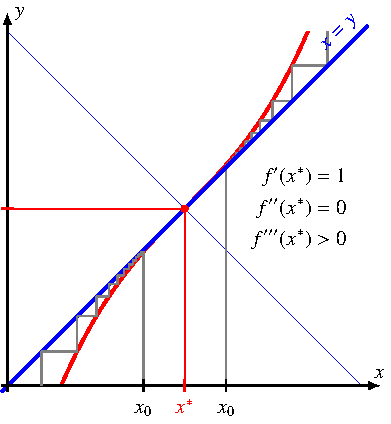
\includegraphics{chapters/10-arithmetik/figures/m1kp.pdf}
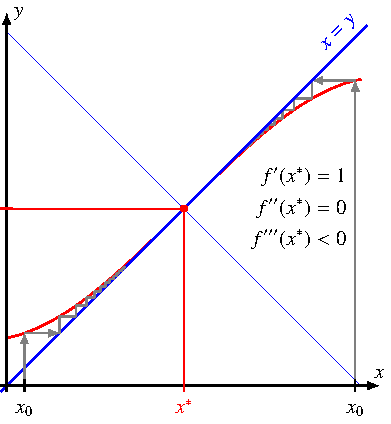
\includegraphics{chapters/10-arithmetik/figures/m1kn.pdf}
\caption{Die Fixpunktiteration $x_{n+1}=f(x_n)$ mit Fixpunkt $x^*$
mit $f'(x^*)=1$ und $f''(x^*)=0$ divergiert für $f'''(x^*)>0$
und konvergiert sehr langsam für $f'''(x^*)<0$.
\label{buch:figure:fixpunkt:abl1kub}}
\end{figure}
%
\begin{figure}
\centering
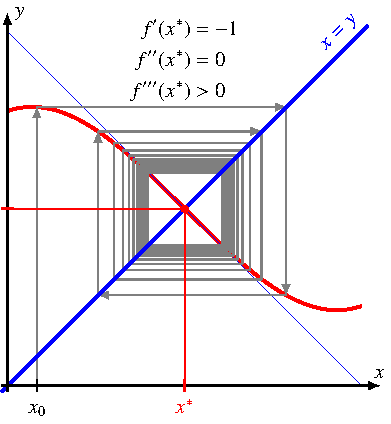
\includegraphics{chapters/10-arithmetik/figures/mnkp.pdf}
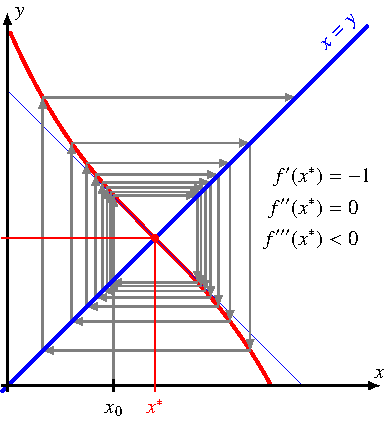
\includegraphics{chapters/10-arithmetik/figures/mnkn.pdf}
\caption{Die Fixpunktiteration $x_{n+1}=f(x_n)$ mit Fixpunkt $x^*$
mit $f'(x^*)=-1$ und $f''(x^*)=0$ konvergiert sehr langsam für $f'''(x^*)>0$
und divergiert für $f'''(x^*)<0$.
\label{buch:figure:fixpunkt:ablm1kub}}
\end{figure}
%
Alle möglichen Situationen sind in den
Abbildungen~\ref{buch:figure:fixpunkt:abl1kub} und
\ref{buch:figure:fixpunkt:ablm1kub} dargestellt.

Wir gehen also davon aus, dass sich $f$ in einer Umgebung von $x^*$
in der Form
\[
f(x^*+\delta)
\simeq
\tilde{f}(x^*+\delta)
=
x^* + f'(x^*)\delta + \frac1{6}f'''(x^*) \delta^3
=
x^* + s\delta + a\delta^3
\]
entwickeln lässt, wobei $s=\pm 1$ und $a\ne 0$ ist.

Der Iterationsfehler $\delta_{n+1}$ verhält sich wie
\begin{align*}
x^* + \delta_{n+1}
&=
f(x_n)
=
f(x^* + \delta_n)
=
x^* + s\delta_n + a\delta_n^3 + O(\delta_n^4).
\\
\delta_{n+1}
&=
s\delta_n + a\delta_n^3 + O(\delta_n^4)
=
\delta_n(s+a\delta_n^2) + O(\delta_n^4)
=
s\delta_n\biggl(1+\frac{a}{s}\delta_n^2\biggr) + O(\delta_n^4)
\end{align*}
Da $\delta_n^2>0$ ist, ist der Klammerausdruck genügend nahe bei $x^*$
immer positiv.
Der Betrag des Fehlers verhält sich dann wie
\[
|\delta_{n+1}|
=
|\delta_n| \cdot \biggl(1 + \frac{a}{s}\delta_n^2\biggr) + O(\delta_n^4).
\]
Ob der Fehler bei der Iteration grösser oder kleiner wird, hängt also
einzig vom Vorzeichen von $a/s$ ab.
Ist $a/s > 0$, wird der Fehler grösser, die Iterationsfolge ist divergent,
ist $a/s < 0$, wird der Fehler kleiner, die Iterationsfolge konvergiert.
Wir fassen diese Resultate zusammen im folgenden Satz.

\begin{satz}
Falls $f\colon\mathbb R\to\mathbb R$ den Fixpunkt $x^*\in\mathbb R$ hat,
und $f'(x^*)=\pm1$, $f''(x^*)=0$ und $f'''(x^*)\ne 0$ ist, dann ist die
Iterationsfolge $x_{n+1}=f(x_n)$ konvergent, falls $f'(x^*)\cdot f'''(x^*)<0$
ist, gleichbedeutend damit, wenn $f'(x^*)$ und $f'''(x^*)$ verschiedene
Vorzeichen haben.
Wenn $f'(x^*)$ und $f'''(x^*)$ das gleiche Vorzeichen haben, dann ist
die Fixpunktiterationsfolge divergent.
\end{satz}

Abbildung~\ref{buch:figure:fixpunkt:abl1kub} zeigt die Situation $f'(x^*)=1$
während Abbildung~\ref{buch:figure:fixpunkt:ablm1kub} die Situation
$f'(x^*)=-1$ abdeckt.


%
% instabilitaet.tex
%
% (c) 2020 Prof Dr Andreas Müller, Hochschule Rapperswil
%
\section{Numerische Instabilität
\label{buch:section:instabilitaet}}
\rhead{Numerische Instabilitöt}
\index{numerische Instabilität}%
\index{Instabilität}%
Die Untersuchungen zum Verhalten von Iterationsfolgen sind davon
ausgegangen, dass alle Rechnung ohne Fehler ausgeführt werden können.
\index{Iterationsfolge}%
Dies ist aber nicht realistisch, in den meisten numerischen Berechnungen
müssen Zwischenresultate mit der beschränkten verfügbaren Genauigkeit
der Gleitkommaformate gespeichert werden, die die Maschine zur Verfügung
stellt.
\index{Konvergenz}%
Es ist daher zu untersuchen, wie sich die Konvergenz eines Lösungsverfahrens
ändert, wenn es durch Rundungsfehler im Laufe der Rechnung gestört wird.
\index{Rundungsfehler}%

%
% Eine instabile Quadratwurzel
%
\subsection{Eine instabile Quadratwurzel
\label{buch:subsection:quadratwurzel}}
Die Quadratwurzel von $a$ ist ein Fixpunkt der Funktion
$f(x)=x^3/a$ denn $f(\!\sqrt{a})=a^{\frac32}/a=\!\sqrt{a}$.
\index{Quadratwurzel}%
\index{Wurzel}%
Das Konvergenzkriterium Satz~\ref{buch:satz:konvergenzkriterium} besagt,
dass Konvergenz garantiert ist, wenn der Betrag der Ableitung von $f'(x)$
am Fixpunkt kleiner als $1$ ist.
\index{Ableitung}%
Aber
\[
f'(x) = \frac{3x^2}{a}
\quad\Rightarrow\quad
f'(\!\sqrt{a}) = \frac{3\!\sqrt{a}^2}{a}=3,
\]
die Iterationsfolge wird also niemals konvergieren.
Im Gegenteil, der Fehler wird in jeder Iteration um den Faktor $3$
anwachsen.

Der \texttt{float}-Gleitkommatyp verwendet eine Mantisse von 23 bit,
das niederwertigste Bit hat also die Wertigkeit $2^{-23}$.
Eine Approximation von $\!\sqrt{a}$ wird daher, sofern sie nicht
exakt ist, beim Speichern als \texttt{float}-Zahl einen Fehler
von der Grössenordnung $2^{-24}$ aufnehmen.
\index{Approximation}%
Nach $k$ Iterationen wird dieser Fehler auf $3^k2^{-24}=2^{k\log_23-24}$
angewachsen sein.
\index{Iteration}%
Nach $k\ge 24/\log_23=15.142$ Iterationen ist also der Fehler von der
gleichen Grössenordnung wie das gesuchte Resultat.

\begin{table}
\centering
\renewcommand\arraystretch{1.15}
\begin{tabular}{|
>{$}r<{$}|
>{$}r<{$}|
>{$}r<{$}|
>{$}r<{$}|
>{$}r<{$}|
>{$}r<{$}|}
\hline
  & \texttt{10001} & \texttt{10010} & \texttt{10011} & \texttt{10100} & \texttt{10101} \\
  &   1.414213 &   1.414213 &   1.414214 &   1.414214 &   1.414214 \\
  & -2.384\cdot 10^{-7} & -1.192\cdot 10^{-7} &          0 & 1.192\cdot 10^{-7} & 2.384\cdot 10^{-7} \\
\hline
 1&   1.414213 &   1.414213 &   1.414213 &   1.414214 &   1.414214 \\
 2&   1.414211 &   1.414212 &   1.414213 &   1.414214 &   1.414216 \\
 3&   1.414207 &   1.414210 &   1.414212 &   1.414216 &   1.414220 \\
 4&   1.414193 &   1.414204 &   1.414210 &   1.414220 &   1.414232 \\
 5&   1.414152 &   1.414184 &   1.414204 &   1.414232 &   1.414268 \\
 6&   1.414029 &   1.414126 &   1.414184 &   1.414268 &   1.414377 \\
 7&   1.413660 &   1.413951 &   1.414126 &   1.414377 &   1.414705 \\
 8&   1.412553 &   1.413427 &   1.413951 &   1.414705 &   1.415687 \\
 9&   1.409239 &   1.411856 &   1.413427 &   1.415687 &   1.418640 \\
10&   1.399341 &   1.407152 &   1.411856 &   1.418640 &   1.427533 \\
11&   1.370064 &   1.393135 &   1.407152 &   1.427533 &   1.454550 \\
12&   1.285858 &   1.351915 &   1.393135 &   1.454550 &   1.538706 \\
13&   1.063039 &   1.235429 &   1.351915 &   1.538706 &   1.821534 \\
14&   0.600645 &   0.942808 &   1.235429 &   1.821534 &   3.021912 \\
15&   0.108348 &   0.419024 &   0.942808 &   3.021912 &  13.797982 \\
16&6.359\cdot 10^{-\phantom{0}4}&3.678\cdot 10^{-\phantom{0}2}&   0.419024 &  13.797982 &1.313\cdot10^{\phantom{0}3}\\
17&1.286\cdot 10^{-10}&2.489\cdot 10^{-\phantom{0}5}&3.678\cdot 10^{-\phantom{0}2}&1.313\cdot10^{\phantom{0}3}&1.132\cdot10^{\phantom{0}9}\\
18&1.063\cdot 10^{-30}&7.710\cdot 10^{-15}&2.489\cdot 10^{-5\phantom{0}}&1.132\cdot10^{\phantom{0}9}&7.271\cdot10^{26}\\
19&  0.000000  &2.298\cdot 10^{-43}&7.710\cdot 10^{-15}&7.271\cdot10^{26}&  \infty    \\
20&  0.000000  &  0.000000  &2.298\cdot 10^{-43}&  \infty    &  \infty    \\
\hline
\end{tabular}
\caption{Iterationsfolge der Funktion $f(x)=x^3/2$ für verschiedene Näherungen
des Fixpunktes $x^*=\!\sqrt{2}$.
Die Startwerte unterscheiden sich nur in den letzten zwei Bits ihrer
Darstellung als \texttt{float}-Gleitkommazahl, die letzten fünf Bits
der Mantisse sind in der ersten Kopfzeile dargestellt.
In der dritten Zeile stehen die Differenzen zur besten Approximation
von $\!\sqrt{2}$ durch eine \texttt{float}-Zahl.
\label{buch:table:sqrtinstabil}}
\end{table}

Wir illustrieren dies mit einer Rechnung\footnote{Das C++-Programm
hierzu ist \texttt{sqrt.cpp} im Verzechnis
\texttt{buch/chapters/experimente/sqrt} von \cite{buch:repo}.},
deren Resultate in Tabelle~\ref{buch:table:sqrtinstabil} zusammengestellt
sind.
\index{C++}%
Zunächst berechnen wir die Quadratwurzel $\!\sqrt{2}$ als \texttt{float}-Zahl.
Dann bilden wir die nächsten Nachbarn, die sich nur in den letzten
zwei Bits unterscheiden, die letzten fünf Bits der Mantisse dieser
Zahlen sind in der obersten Kopfzeile der Tabelle gezeigt.
In der zweiten Kopfzeile sieht man, dass diese Unterschiede so klein
sind, dass sie nur gerade die Rundung in der sechsten dezimalen
Nachkommastelle beinflussen können.
Der Unterschied dieser Startwerte zum Maschinen-Wert für $\!\sqrt{2}$
ist in der dritten Kopfzeile dargestellt.

Im unteren Teil der Tabelle wird dann ausgehend von jedem dieser Startwerte
die Iterationsfolge mit der Funktion $f(x)=x^3/2$ gebildet.
\index{Startwert}%
Spätestens nach der zweiten Iteration beginnen sich die Werte vom Fixpunkt zu
entfernen, nach 16 Iterationen sind die Abweichungen von der 
Grössenordnung $1$ wie in der Überschlagsrechnung weiter oben
vorhergesagt.

%
% Numerische Instabilität
%
\subsection{Numerische Instabilität
\label{buch:subsection:numerischeinstabilitaet}}
Von {\em numerischer Instabilität} spricht man, wenn ein Berechnungsverfahren
\index{Instabilität!numerisch}%
\index{numerische Instabilität}%
allein wegen der unvermeidlichen Rundungsfehler keine sinnvollen
Resultate liefern kann.

\begin{beispiel}
Es soll das Integral
\[
I_n = \int_0^1 \frac{x^n}{x+a}\,dx
\]
für festes $a>1$ und für ganze Zahlen $n$ mit $1\le n\le 15$ berechnet
werden.
\index{Integral}%
Da im Intervall $[0,1]$ gilt $x^{n+1}>x^n$ ist $I_n$ eine monoton
abnehmende Folge.
Es ist auch klar, dass $\lim_{n\to\infty}I_n=0$.

Das Integral ist im Prinzip nicht schwierig zu berechnen, wenn man im
Integranden die Polynomdivision ausführt:
\index{Polynomdivision}%
\begin{align}
\frac{x^n}{x+a}
&=
x^{n-1} -ax^{n-2}+a^2x^{n-3}-\dots +(-1)^n xa^{n-2} +(-1)^{n-1}a^{n-1}
+(-1)^n\frac{a^n}{a+x}
\notag
\\
\int_0^1 \frac{x^n}{x+a}\,dx
&=
\frac1n
-\frac{a}{n-1}
+\frac{a^2}{n-2}
-\dots
+(-1)^n\frac{a^{n-2}}{2}
+(-1)^{n-1}a^{n-1}
+\log(1+a)-\log a.
\label{buch:numerik:instabil:summe}
\end{align}
Jeder Term ist ein elementares Integral.
\end{beispiel}

\begin{table}
\centering
\renewcommand\arraystretch{1.15}
\begin{tabular}{|>{$}r<{$}|>{$}r<{$}|>{$}r<{$}|}
\hline
 n&   I_n   & \text{Rückwärtsiteration}\\
\hline
 0&   0.095310179804324{\color{red}9          } & 0.09531017980432486\\
 1&   0.04689820195675{\color{red}07          } & 0.04689820195675140\\
 2&   0.0310179804324{\color{red}935          } & 0.03101798043248600\\
 3&   0.023153529008{\color{red}3985          } & 0.02315352900847329\\
 4&   0.01846470991{\color{red}60155          } & 0.01846470991526711\\
 5&   0.0153529008{\color{red}398455          } & 0.01535290084732894\\
 6&   0.013137658{\color{red}2682119          } & 0.01313765819337729\\
 7&   0.01148056{\color{red}01750236          } & 0.01148056092337000\\
 8&   0.01019439{\color{red}82497636          } & 0.01019439076629997\\
 9&   0.009167{\color{red}1286134746          } & 0.00916720344811137\\
10&   0.00832{\color{red}87138652537          } & 0.00832796551888631\\
11&   0.00762{\color{red}19522565537          } & 0.00762943572022779\\
12&   0.007{\color{red}1138107677959          } & 0.00703897613105546\\
13&   0.00{\color{red}57849692451174          } & 0.00653331561252233\\
14&   0.0{\color{red}135788789773972          } & 0.00609541530334817\\
15&  -0.0{\color{red}691221231073049          } & 0.00571251363318499\\
16&   0.{\color{red}753721231073049\phantom{0}} & 0.00537486366815009\\
17&  {\color{red}-7.47838878131872\phantom{00}} & 0.00507489273026384\\
18&  {\color{red}74.8394433687428\phantom{000}} & 0.00480662825291712\\
19&{\color{red}-748.341802108480\phantom{0000}} & 0.00456529641819719\\
20&{\color{red}7483.46802108480\phantom{00000}} & 0.00434703581802811\\
\hline
\end{tabular}
\caption{Instabile Iteration zur Berechnung der Integrale $I_n$ mit
$a=10$.
In jedem Schritt wird der Fehler mit $a$ multipliziert.
In der dritten Spalte die Resultate der stabilen Rückwärtsiteration.
\index{Rückwärtsiteration}%
\label{buch:table:Iiteration}}
\end{table}

Wenn $n$ gross ist, ist \eqref{buch:numerik:instabil:summe}
eine ziemlich aufwendig Rechnung.
Da man das Integral für alle $n$ haben will, bietet sich eine
Rekursionsformel an.
\index{Rekursionsformel}%
Es ist nämlich
\begin{align*}
I_n
&=
\int_0^1 \frac{x^n}{x+a}\,dx
=
\int_0^1 \frac{x^{n-1}(x+a-a)}{x+a}\,dx
=
\int_0^1 x^n - \frac{ax^{n-1}}{x+a}\,dx
\\
&=
\int_0^1 x^n\,dx - aI_{n-1}
=
\frac1{n+1} - a I_{n-1}.
\end{align*}
Wenn man also $I_0$ berechnet hat, dann kann man mit dieser 
Rekursionsformel alle anderen $I_n$ berechnen.
$I_0$ ist nicht schwierig zu berechnen, es ist
\[
I_0 = \int_0^1 \frac{1}{x+a}\,dx = \log(1+a) - \log a = \log\frac{1+a}a.
\]

Um die Empfindlichkeit der Rekursion auf Rundungsfehler zu untersuchen,
nehmen wir vereinfachend an, dass ausschliesslich bei der Berechnung von
$I_0$ ein unvermeidlicher Rundungsfehler der Grösse $\varepsilon$ passiert
und dass alle folgenden Operationen exakt ausgeführt werden können.
Da der Logarithmus eine transzendente Funktion ist, werden fast alle Werte
des Logrithmus bei Speichern als Gleitkommazahl gerundet werden müssen.
\index{Logarithmus}%
Wir müssen jetzt also die Rekursionsfolge $I^*_n$ ausgehend von
$I_0^* = I_0+\varepsilon$
bilden:
\[
\begin{aligned}
I_0^* &= I_0 + \varepsilon
\\
I_1^* &= \frac12 - a(I_0^*) = \frac12-aI_0 - a\varepsilon
      &&=I_1 - a \varepsilon
\\
I_2^* &= \frac13 - a(I_1^*) = \frac13-aI_1 + a^2\varepsilon
      &&=I_2 + a^2 \varepsilon
\\
\vdots\;&\quad\vdots\\
I_n^* &= \frac{1}{n+1} -aI_{n-1}^* = \frac{1}{n+1} - aI_{n-1} + (-a)^n\varepsilon
      &&= I_{n-1} + (-a)^n\varepsilon.
\end{aligned}
\]
In jedem Iterationsschritt wird der Fehler mit $a$ multipliziert.
In jedem Schritt gehen als $\log_2a$ Binärstellen Genaugikeit verloren.
Für $a=10$ bedeutet dies, dass in jedem Schritt eine Dezimalstelle
verloren geht.

Die Instabilität rührt daher, dass der Fehler in jedem Schritt mit
$a>1$ multipliziert wird.
Wir könnten versuchen, die Rekursion umzukehren, so dass durch $a$ 
dividiert wird, so könnte das Problem möglicherweise behoben werden.
Indem wir nach $I_{n-1}$ auflösen, erhalten wir die Rekursionsformel
\[
I_{n-1} = \frac1{a} \biggl(
\frac{1}{n+1} -I_n\biggr).
\]
\index{Rekursionsformel}%
In dieser Rekursion wird tatsächlich in jedem Schritt durch $a$ dividiert,
man darf daher davon ausgehen, dass in jeder Iteration 
$\log_2a$ Binärstellen Genauigkeit gewonnen werden.

Allerdings muss man für diese Iteration einen der Werte $I_n$ bereits
kennen.
Man weiss aber, dass $\lim_{n\to\infty} I_n=0$ ist, d.~h.~wenn man
$I_n$ durch $0$ ersetzt macht man einen Fehler exakt von der
Grössenordnung $I_n$.
Die Rekursion reduziert diesen Fehler in jedem Schritt um $\log_2a$
Binärstellen.
Da die Werte $I_n$ alle kleiner als $1$ sind, macht man also
niemals einen Fehler grösser als $1$ und nach $k$ Rückwärtsiterationsschritten
ist der Fehler kleiner als $a^k$.
\index{Rückwärtsiteration}%
Man kann also selbst ohne die Kenntnis eines Startwertes ausreichend
genaue Werte von $I_n$ bestimmen.
\index{Startwert}%
Dies ist in der dritten Spalte von Tabelle~\ref{buch:table:Iiteration}
durchgeführt.






%
% kondition.tex
%
% (c) 2020 Prof Dr Andreas Müller, Hochschule Rapperswil
%
\section{Kondition
\label{buch:section:kondition}}
Die Diskussion der iterativen Verfahren in
Abschnitt~\ref{buch:section:gaussseidel} hat gezeigt, dass
der Spektralradius aus Definition~\ref{buch:definition:spektralradius}
Auskunft gibt darüber, ob ein iteratives Verfahren konvergiert.
\index{Spektralradius}%
Insbesondere wurde behauptet, dass Spektralradius $\varrho(M)$ und
Gelfand-Radius $\pi(M)$ übereinstimmen.
In diesem Abschnitt sollen diese Kennzahl noch etwas vertieft
untersucht werden.

%
% Gelfand-Radius und Eigenwerte
%
\subsection{Gelfand-Radius und Eigenwerte
\label{buch:subsection:spektralradius}}
In Abschnitt~\ref{buch:subsection:konvergenzbedingung}
ist der Gelfand-Radius mit Hilfe eines Grenzwertes definiert worden.
\index{Gelfand-Radius}%
Nur dieser Grenzwert ist in der Lage, über die Konvergenz eines 
Iterationsverfahrens Auskunft zu geben.
Der Grenzwert ist aber sehr mühsam zu berechnen.
\index{Grenzwert}%
Es wurde angedeutet, dass der Gelfand-Radius mit dem Spektralradius
übereinstimmt, dem Betrag des des betragsgrössten Eigenwertes.
Dies hat uns ein vergleichsweise einfach auszuwertendes Konvergenzkriterium
geliefert.
\index{Konvergenzkriterium}%
In diesem Abschnitt soll diese Identität zunächst an Spezialfällen
und später ganz allgemein gezeigt werden.

\subsubsection{Spezialfall: Diagonalisierbare Matrizen}
Ist eine Matrix $A$ diagonalisierbar, dann kann Sie durch eine Wahl
einer geeigneten Basis in Diagonalform
\index{diagonalisierbar}%
\index{Diagonalform}%
\[
A'
=
\begin{pmatrix}
\lambda_1&        0&\dots &0\\
0        &\lambda_2&\dots &0\\
\vdots   &         &\ddots&\vdots\\
0        &        0&\dots &\lambda_n
\end{pmatrix}
\]
gebracht werden, wobei die Eigenwerte $\lambda_i$  möglicherweise auch
komplex sein können.
\index{komplex}%
Die Bezeichnungen sollen so gewählt sein, dass $\lambda_1$ der
betragsgrösste Eigenwert ist, dass also
\[
|\lambda_1| \ge |\lambda_2| \ge \dots \ge |\lambda_n|.
\]
Wir nehmen für die folgende, einführende Diskussion ausserdem an, dass
sogar $|\lambda_1|>|\lambda_2|$ gilt.

Unter den genannten Voraussetzungen kann man jetzt den Gelfand-Radius
von $A$ berechnen.
Dazu muss man $|A^nv|$ für einen beliebigen Vektor $v$ und für
beliebiges $n$ berechnen.
Der Vektor $v$ lässt sich in der Eigenbasis von $A$ zerlegen, also
als Summe
\index{Eigenbasis}%
\[
v = v_1+v_2+\dots+v_n
\]
schreiben, wobei $v_i$ Eigenvektoren zum Eigenwert $\lambda_i$ sind oder
Nullvektoren.
Die Anwendung von $A^k$ ergibt dann
\[
A^k v
=
A^k v_1 + A^k v_2 + \dots + A^k v_n
=
\lambda_1^k v_1 + \lambda_2^k v_2 + \dots + \lambda_n^k v_n.
\]
Für den Grenzwert braucht man die Norm von $A^kv$, also
\begin{align}
|A^kv|
&= |\lambda_1^k v_1 + \lambda_2^k v_2 + \dots + \lambda_3 v_3|
\notag
\\
\Rightarrow\qquad
\frac{|A^kv|}{\lambda_1^k}
&=
\biggl|
v_1 +
\biggl(\frac{\lambda_2}{\lambda_1}\biggr)^k v_2
+
\dots
+
\biggl(\frac{\lambda_n}{\lambda_1}\biggr)^k v_n
\biggr|.
\label{buch:spektralradius:eqn:eigenwerte}
\end{align}
Da alle Quotienten $|\lambda_i/\lambda_1|<1$ sind für $i\ge 2$,
konvergieren alle Terme auf der rechten Seite von
\eqref{buch:spektralradius:eqn:eigenwerte}
ausser dem ersten gegen $0$.
Folglich ist
\[
\lim_{k\to\infty} \frac{|A^kv|}{|\lambda_1|^k}
=
|v_1|
\qquad\Rightarrow\qquad
\lim_{k\to\infty} \frac{|A^kv|^\frac1k}{|\lambda_1|}
=
\lim_{k\to\infty}|v_1|^{\frac1k}
=
1.
\]
Dies gilt für alle Vektoren $v$, für die $v_1\ne 0$ ist.
Der maximale Wert dafür wird erreicht, wenn man für 
$v$ einen Eigenvektor der Länge $1$ zum Eigenwert $\lambda_1$ einsetzt,
dann ist $v=v_1$.
Es folgt dann
\[
\pi(A)
=
\lim_{k\to\infty} \| A^k\|^\frac1k
=
\lim_{k\to\infty} |A^kv|^\frac1k
=
|\lambda_1|
=
\varrho(A).
\]
Damit ist gezeigt, dass im Spezialfall einer diagonalisierbaren Matrix der
Gelfand-Radius tatsächlich der Betrag des betragsgrössten Eigenwertes ist.
\index{Gelfand-Radius}%

\subsubsection{Blockmatrizen}
Wir betrachten jetzt eine $(n+m)\times(n+m)$-Blockmatrix der Form
\begin{equation}
A = \begin{pmatrix} B & 0 \\ 0 & C\end{pmatrix}
\label{buch:spektralradius:eqn:blockmatrix}
\end{equation}
mit einer $n\times n$-Matrix $B$ und einer $m\times m$-Matrix $C$.
Ihre Potenzen haben ebenfalls Blockform:
\[
A^k = \begin{pmatrix} B^k & 0 \\ 0 & C^k\end{pmatrix}.
\]
Ein Vektor $v$ kann in die zwei Summanden $v_1$ bestehen aus den
ersten $n$ Komponenten und $v_2$ bestehen aus den letzten $m$ 
Komponenten zerlegen.
Dann ist
\[
A^kv = B^kv_1 + C^kv_2.
\qquad\Rightarrow\qquad
|A^kv|
\le
|B^kv_1| + |C^kv_2|
\le 
\pi(B)^k |v_1| + \pi(C)^k |v_2|.
\]
Insbesondere haben wir das folgende Lemma gezeigt:

\begin{lemma}
\label{buch:spektralradius:lemma:diagonalbloecke}
Eine diagonale Blockmatrix $A$ \eqref{buch:spektralradius:eqn:blockmatrix}
Blöcken $B$ und $C$  hat Gelfand-Radius
\[
\pi(A) = \max ( \pi(B), \pi(C) )
\]
\end{lemma}

Selbstverständlich lässt sich das Lemma auf Blockmatrizen mit beliebig
vielen diagonalen Blöcken verallgemeinern.
\index{Blockmatrix}%

Für Diagonalmatrizen der genannten Art sind aber auch die 
Eigenwerte leicht zu bestimmen.
\index{Diagonalmatrix}%
Hat $B$ die Eigenwerte $\lambda_i^{(B)}$ mit $1\le i\le n$ und $C$ die
Eigenwerte $\lambda_j^{(C)}$ mit $1\le j\le m$, dann ist das charakteristische
Polynom der Blockmatrix $A$ natürlich
\index{charakteristisches Polynom}%
\index{Polynom!charakteristisch}%
\[
\chi_A(\lambda) = \chi_B(\lambda)\chi_C(\lambda),
\]
woraus folgt, dass die Eigenwerte von $A$ die Vereinigung der Eigenwerte
von $B$ und $C$ sind.
Daher gilt auch für die Spektralradius die Formel
\[
\varrho(A) = \max(\varrho(B) , \varrho(C)).
\]

\subsubsection{Jordan-Blöcke}
\index{Jordan-Block}%
Nicht jede Matrix ist diagonalisierbar, die bekanntesten Beispiele sind
die Matrizen
\begin{equation}
J_n(\lambda)
=
\begin{pmatrix}
\lambda &      1&       &       &       &       \\
        &\lambda&      1&       &       &       \\[-5pt]
        &       &\lambda&\ddots &       &       \\[-5pt]
        &       &       &\ddots &      1&       \\
        &       &       &       &\lambda&      1\\
        &       &       &       &       &\lambda
\end{pmatrix},
\label{buch:spektralradius:eqn:jordan}
\end{equation}
wobei $\lambda\in\mathbb C$ eine beliebige komplexe Zahl ist.
Wir nennen diese Matrizen {\em Jordan-Matrizen}.
Es ist klar, dass $J_n(\lambda)$ nur den $n$-fachen Eigenwert
$\lambda$ hat und dass der erste Standardbasisvektor ein
Eigenvektor zu diesem Eigenwert ist.

In der linearen Algebra lernt man, dass jede Matrix durch Wahl
\index{lineare!Algebra}%
einer geeigneten Basis als Blockmatrix der Form
\[
A
=
\begin{pmatrix}
J_{n_1}(\lambda_1) &        0         & \dots & 0 \\
       0         & J_{n_2}(\lambda_2) & \dots & 0 \\[-4pt]
\vdots           &\vdots            &\ddots &\vdots \\
       0         &        0         & \dots &J_{n_l}(\lambda_l)
\end{pmatrix}
\]
geschrieben werden kann\footnote{Sofern die Matrix komplexe Eigenwerte
hat muss man auch komplexe Basisvektoren zulassen.}.
Die früheren Beobachtungen über den Spektralradius und den
Gelfand-Radius von Blockmatrizen zeigen uns daher, dass
nur gezeigt werden muss, dass nur die Gleichheit des Gelfand-Radius
und des Spektral-Radius von Jordan-Blöcken gezeigt werden muss.

\subsubsection{Iterationsfolgen}
\begin{satz}
\label{buch:spektralradius:satz:grenzwert}
Sei $A$ eine $n\times n$-Matrix mit Spektralradius $\varrho(A)$.
Dann ist $\varrho(A)<1$ genau dann, wenn
\[
\lim_{k\to\infty} A^k = 0.
\]
Ist andererseits $\varrho(A) > 1$, dann ist
\[
\lim_{k\to\infty} \|A^k\|=\infty.
\]
\end{satz}

\begin{proof}[Beweis]
Wie bereits angedeutet reicht es, diese Aussagen für einen einzelnen
Jordan-Block mit Eigenwert $\lambda$ zu beweisen.
Die $k$-te Potenz von $J_n(\lambda)$ ist
\[
J_n(\lambda)^k
=
\renewcommand\arraystretch{1.35}
\begin{pmatrix}
\lambda^k    & \binom{k}{1} \lambda^{k-1} & \binom{k}{2}\lambda^{k-2}&\dots&
\binom{k}{n-1}\lambda^{k-n+1}\\
      0      &\lambda^k & \binom{k}{1} \lambda^{k-1} & \dots &\binom{k}{n-2}\lambda^{k-n+2}\\
      0     &      0    & \lambda^k & \dots &\binom{k}{n-k+3}\lambda^{k-n+3}\\
\vdots      & \vdots    &               &\ddots & \vdots\\
     0      &      0    &      0        &\dots  &\lambda^k
\end{pmatrix}.
\]
Falls $|\lambda| < 1$ ist, gehen alle Potenzen von $\lambda$ exponentiell
schnell gegen $0$, während die Binomialkoeffizienten nur polynomiell
schnell anwachsen. 
\index{Binomialkoeffizient}
In diesem Fall folgt also $J_n(\lambda)\to 0$.

Falls $|\lambda| >1$ divergieren bereits die Elemente auf der Diagonalen,
also ist $\|J_n(\lambda)^k\|\to\infty$ mit welcher Norm auch immer man
man die Matrix misst.
\end{proof}

Aus dem Beweis kann man noch mehr ablesen.
Für $\varrho(A)< 1$ ist die Norm $ \|A^k\| \le M \varrho(A)^k$ für eine
geeignete Konstante $M$,
für $\varrho(A) > 1$ gibt es eine Konstante $m$ mit
$\|A^k\| \ge m\varrho(A)^k$.

\subsubsection{Der Satz von Gelfand}
Der Satz von Gelfand ergibt sich jetzt als direkte Folge aus dem
Satz~\ref{buch:spektralradius:satz:grenzwert}.

\begin{satz}[Gelfand]
\index{Satz von Gelfand}
\index{Gelfand!Satz von}
\label{buch:satz:gelfand}
Für jede komplexe $n\times n$-Matrix $A$ gilt
\[
\pi(A)
=
\lim_{k\to\infty}\|A^k\|^\frac1k
=
\varrho(A).
\]
\end{satz}

\begin{proof}[Beweis]
Der Satz~\ref{buch:spektralradius:satz:grenzwert} zeigt, dass der
Spektralradius ein scharfes Kriterium dafür ist, ob $\|A^k\|$ 
gegen 0 oder $\infty$ konvergiert.
Andererseits ändert ein Faktor $t$ in der Matrix $A$ den Spektralradius
ebenfalls um den gleichen Faktor, also $\varrho(tA)=t\varrho(A)$.
Natürlich gilt auch
\[
\pi(tA)
=
\lim_{k\to\infty} \|t^kA^k\|^\frac1k
=
\lim_{k\to\infty} t\|A^k\|^\frac1k
=
t\lim_{k\to\infty} \|A^k\|^\frac1k
=
t\pi(A).
\]

Wir betrachten jetzt die Matrix
\[
A(\varepsilon) = \frac{A}{\varrho(A) + \varepsilon}.
\]
Der Spektralradius von $A(\varepsilon)$ ist
\[
\varrho(A(\varepsilon)) = \frac{\varrho(A)}{\varrho(A)+\varepsilon},
\]
er ist also $>1$ für negatives $\varepsilon$ und $<1$ für positives
$\varepsilon$.
Aus dem Satz~\ref{buch:spektralradius:satz:grenzwert} liest man daher ab,
dass $\|A(\varepsilon)^k\|$ genau dann gegen $0$ konvergiert, wenn
$\varepsilon > 0$ ist und divergiert genau dann, wenn $\varepsilon< 0$ ist.

Aus der Bemerkung nach dem Beweis von
Satz~\ref{buch:spektralradius:satz:grenzwert} schliesst man daher, dass 
es im Fall $\varepsilon > 0$ eine Konstante $M$ gibt mit
\begin{align*}
\|A(\varepsilon) ^k\|\le M\varrho(A(\varepsilon))^k
\quad&\Rightarrow\quad
\|A(\varepsilon) ^k\|^\frac1k\le M^\frac1k\varrho(A(\varepsilon))
\\
&\Rightarrow\quad
\pi(A) \le  \varrho(A(\varepsilon))
\underbrace{\lim_{k\to\infty} M^\frac1k}_{\displaystyle=1}
=
\varrho(A(\varepsilon))
=
\varrho(A)+\varepsilon.
\end{align*}
Dies gilt für beliebige $\varepsilon >0$, es folgt daher
$\pi(A) \le \varrho(A)$.

Andererseits gibt es für $\varepsilon <0$ eine Konstante $m$ mit
\begin{align*}
\|A(\varepsilon) ^k\|\ge m\varrho(A(\varepsilon))^k
\quad&\Rightarrow\quad
\|A(\varepsilon) ^k\|^\frac1k\ge m^\frac1k\varrho(A(\varepsilon))
\\
&\Rightarrow\quad
\pi(A) \ge  \varrho(A(\varepsilon))
\underbrace{\lim_{k\to\infty} m^\frac1k}_{\displaystyle=1}
=
\varrho(A(\varepsilon))
=
\varrho(A)+\varepsilon.
\end{align*}
Dies gilt für beliebige $\varepsilon> 0$, es folgt daher
$\pi(A) \ge \varrho(A)$.
Zusammen mit $\pi(A) \le \varrho(A)$ folgt $\pi(A)=\varrho(A)$.
\end{proof}

%
% Konditionszahl
%
\subsection{Konditionszahl
\label{buch:subsection:konditionszahl}}
\index{Konditionszahl}%
Der Spektralradius $\varrho(A)$ einer Matrix $A$ gibt darüber Auskunft,
ob ein auf $A$ basierendes Iterationsverfahren konvergiert.
Er sagt aber nicht einmal, ob die Matrix zum Beispiel regulär.
Doch auch diese Information lässt sich aus den Eigenwerten ablesen.
Die Matrix ist genau dann regulär, wenn alle Eigenwerte von $0$ verschieden
sind.
Ein Problem entsteht also dann, wenn einzelne Eigenwerte sehr klein sind.
Die Kombination besonders grosser und besonders kleiner Eigenwerte 
ist also ein Indikator, der auf mögliche numerische Probleme hinweisen kann.

Die Eigenwerte von $A^{-1}$ sind die Reziproken der Eigenwerte von $A$.
Ist $\lambda$ ein Eigenwert von $A$, dann ist $\lambda^{-1}$ ein Eigenwert
von $A^{-1}$.
Der betragskleinste Eigenwert von $A$ ist der betragsgrösste Eigenwert von
$A^{-1}$.
Numerische Probleme werden also dadurch angezeigt, dass $\varrho(A)$ gross
ist, oder $\varrho(A^{-1})$ klein.

\begin{definition}
\label{buch:konditionszahl:definition}
\index{Konditionszahl}%
Die Konditionszahl einer Matrix $A$ ist der Quotient
\[
\kappa(A)
=
\frac{\varrho(A)}{\varrho(A^{-1})}
=
\frac{|\lambda_1|}{|\lambda_n|},
\]
wenn $\lambda_1$ der betragsgrösste und $\lambda_n$ der betragskleinste
Eigenwert von $A$ ist.
\end{definition}

Die Konditionszahl ist also immer $\ge 1$, dieser minimale Wert $1$
wird zum Beispiel für die Einheitsmatrix erreicht.
Schlechte Kondition tritt auf, wenn die Eigenwerte sehr grosse
Betragsunterschiede aufweisen.
\index{Kondition!schlecht}

\begin{beispiel}
Die Kahan-Matrix
\index{Kahan-Matrix}%
\[
A
=
\begin{pmatrix}
1000&999\\
999&998
\end{pmatrix}
\]
besteht aus zwei fast gleichen Zeilen, sie ist als fast singulär,
die Determinante muss sehr klein sein.
Andererseits sind alle Einträge von der Grössenordnung $10^3$, man erwartet
also einen Spektralradius in der selben Grössenordnung.
Die Konditionszahl dürfte daher weit grösser als $10^3$ sein.
Die numerische Rechnung ergibt für die Eigenwerte
\[
\lambda_1 = 1998.00050050375,
\qquad
\lambda_2 = -0.000500500375,
\]
was eine Konditionszahl von
\[
\kappa(A)
\approx
3992006
\approx
4\cdot 10^6
\]
ergibt.
Diese einfache Matrix hat also sehr schlechte Kondition.

Die Determinante von $A$ ist
\index{Determinante}%
\[
\det A
=
1000\cdot 998 -999^2
=
-1.
\]
Damit kann man auch die Inverse algebraisch leicht angeben:
\index{Inverse}%
\[
A^{-1}
=
\frac{1}{\det(A)}
\begin{pmatrix} 998 & -999\\ -999 &1000 \end{pmatrix}.
\]
Die numerische Rechnung offenbart aber die Schwierigkeiten, die die 
schlechte Kondition verursacht.
Das Produkt $AA^{-1}$ müsste die Einheitsmatrix ergeben, die numerische
Rechnung mit dem \texttt{double}-Typ ergibt jedoch
\[
\begin{pmatrix}
   1.0000000000{\color{red}74920} &-0.0000000000{\color{red}52182}\\
   0.00000000000{\color{red}3410} &\phantom{-}1.0000000000{\color{red}20236}
\end{pmatrix},
\]
der numerische Fehler ist also etwa um den Faktor $10^4$ grösser als
bei einer gut konditionierten Matrix erwartet werden kann.
\end{beispiel}



%
% beschleunigung.tex
%
% (c) 2020 Prof Dr Andreas Müller, Hochschule Rapperswil
%
\section{Konvergenzgeschwindigkeit
\label{buch:section:geschwindigkeit}}
\rhead{Konvergenzgeschwindigkeit}
Sind die Fehler einer iterativen numerischen Berechnungsmethoden
bekannt, kann die Gesetzmässigkeit der Fehler ausgenutzt werden,
sie weitgehend zu eliminieren, und so die Konvergenz des Verfahrens
zu beschleunigen.
In diesem Abschnitt wollen wir das Prinzip veranschaulichen, es
soll später im Abschnitt~\ref{buch:section:romberg}
bei der Berechnung von Integralen systematisch angewendet werden.

%
% Lineare und quadratische Konvergenz
%
\subsection{Lineare und quadratische Konvergenz
\label{buch:subsection:linearekonvergenz}}
Wir betrachten zwei Beispiele von Iterationsfolgen genauer, die
deutlich unterschiedlich schnell konvergieren.
Ziel ist, diesen Unterschied zu quantifizieren und ein Kriterium
zu finden, welches schnelle Konvergenz von Iterationsfolgen garantiert.

\subsubsection{Lineare Konvergenz}
Am Beispiel der Iterationsfolge der Funktion $f(x)=\sqrt{x+2}$
von Seite~\pageref{section:beispiel:sqrtiteration}
wurde berechnet, wie sich der Fehler von einer Iteration zur nächsten
entwickelt.
Dabei wurde gefunden, dass der Fehler $\delta_n$ in der $n$-ten Iteration
zu $\delta_{n+1}\approx f'(x^*)\cdot\delta_n$ in der $(n+1)$-ten Iteration
wird.
Sind in der $n$-ten Iteration $k$ Nachkommabits korrekt, ist der Fehler
also von der Grössenordnung $2^{-k}$, wird der Fehler in der $(n+1)$-ten
Iteration von der Grössenordnung $f'(x^*) \cdot 2^{-k}= 2^{-k+\log_2f'(x^*)}$
sein.
In jeder Iteration werden also $\log_2f'(x^*)$ Binärstellen Genauigkeit
gewonnen.

Man sagt, eine Folge ist {\em linear} konvergent, wenn die Anzahl
korrekter Stellen in jeder Iteration um die gleiche Anzahl zunimmt.
Die Anzahl korrekter Stellen wächst in diesem Fall linear mit der
Anzahl Iterationen.

Für eine konvergente Iterationsfolge einer Funktion $f$ liegt also
normalerweise lineare Konvergenz vor, es werden $\log_2 f'(x^*)$
Binärstellen oder $\log_{10}f'(x^3)$ Dezimalstellen Genauigkeit in
jeder Iteration gewonnen.
Falls die Ableitung $f'(x^*)$ verschwindet liegt offenbar ein
Spezialfall vor, er wird im übernächsten Abschnitt genauer untersucht.

\subsubsection{Quadratische Konvergenz}
Ist $x=\sqrt{a}$, dann muss $x = a/x$ gelten, also auch
\[
x = \frac12\biggl(x+\frac{a}x\biggr) = f_a(x).
\]
Mit der Funktion $f_a(x)$ kann man jetzt ein Iterationsfolge konstruieren,
die gegen den Fixpunkt 
\[
x^*=f_a(x^*)
\quad\Rightarrow\quad
x^*=\frac12\biggl(x^*+\frac{a}x^*\biggr)
\quad\Rightarrow\quad
x^{*2}-a=0
\quad\Rightarrow\quad
x^*=\sqrt{a}
\]
von $f_a(x)$ konvergiert.
Wir untersuchen die Konvergenzgeschwindigkeit, indem wir $f_a(x)$
mit Hilfe der Taylor-Reihe approximieren:
\[
f_a(x^*+\delta)
\approx
f_a(x^*) + f_a'(x^*)\cdot\delta + \frac12f''_a(x^*)\cdot\delta^2
\]
Die Ableitungen von $f_a$ sind
\begin{align*}
f'_a(x)
&=
\frac12 -\frac{a}{2x^2}
&&\Rightarrow&
f'_a(x^*)&=0
\\
f''_a(x^*)
&=
\frac{a}{x^3}
&&\Rightarrow&
f''_a(x^*)&=\frac{1}{\!\sqrt{a}}
\end{align*}
Mit $x=x^* =\sqrt{a}$ folgt für den Fehler
\[
f_a(x^*+\delta)
\approx
x^* + \underbrace{\biggl(\frac12-\frac{a}{2x^{*2}}\biggr)}_{\displaystyle=0}\delta
+
\frac{a}{2x^{*3}}\delta^2
=
x^* + \frac{1}{2\sqrt{a}}\delta^2.
\]
Der Fehler wird also im Wesentlichen quadriert.
Sind $k$ Nachkommabits korrekt, liegt ein Fehler von der Grössenordnung
$2^{-k}$ vor. 
Daraus wird in der nächsten Iteration ein Fehler von der Grössenordnung
$2^{-2k}$.
Die Anzahl korrekter Nachkommabits ist $2k$, sie hat sich also
verdoppelt.

Man sagt, eine Folge konvergiert {\em quadratisch} gegen $x^*$,
wenn der Fehler $x_n-x^*$ für $n\to n+1$ quadriert wird, die Anzahl
korrekter Stellen also verdoppelt wird.
Konvergiert eine Folge quadratisch, werden $N$ korrekte Stellen
innert $\log_2N$ Iterationen erreicht.
Quadratische Konvergenz ist also im Vergleich zu linearer Konvergenz
exponentiell schneller und wird daher in Anwendungen angestrebt.

\subsubsection{Konvergenzgeschwindigkeit von Iterationsfolgen}
%
% graphisch2.tex
%
% (c) 2020 Prof Dr Andreas Müller, Hochschule Rapperswil
%
\begin{figure}
\centering
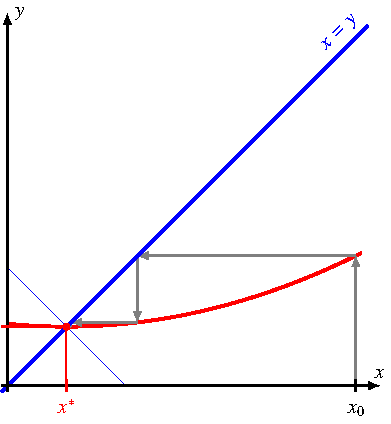
\includegraphics{chapters/10-arithmetik/figures/quadratisch.pdf}
\caption{Die Fixpunktiteration $x_{n+1}=f(x_n)$ konvergiert quadratisch
gegen den Fixpunkt $x^*$
für $f'(x^*)=0$.
\label{buch:figure:fixpunkt:quadratisch}}
\end{figure}

Früher wurde gezeigt, dass die Iterationsfolge $x_{n+1}=f(x_n)$ einer
Funktion $f$ für genügend Nahe bei einem Fixpunkt $x^*$ liegende
Startwerte $x_0$ gegen $x^*$ konvergiert, wenn $|f'(x^*)| < 1$.
Wir sind jetzt auch in der Lage, die Konvergenzgeschwindigkeit
zu quantifizieren.
Dazu entwickeln wird $f(x)$ um $x^*$ bis zur zweiten Ordnung und
erhalten für den Fehler
\begin{equation}
f(x^*+\delta)
\approx
f(x^*) + f'(x^*) \cdot \delta + \frac12f''(x^*)\cdot \delta^2
\label{buch:equation:iterkonv}
\end{equation}
Sofern $f'(x^*)\ne 0$ ist, ist der zweite Term dominant, der Fehler
wird in jeder Iteration mit $f'(x^*)$ multipliziert, es werden in
jeder Iteration $\log_2 f'(x^*)$ Genauigkeit gewonnen.
Es liegt also {\em lineare Konvergenz} vor.
\index{lineare Konvergenz}%
\index{Konvergenz!linear}%

Verschwindet die Ableitung $f'(x^*)=0$, dann fällt der zweite Term
auf der rechten Seite von~\eqref{buch:equation:iterkonv} weg, der
Fehler ist im wesentlich quadratisch kleiner, es liegt {\em quadratische
Konvergenz} vor.
\index{quadratische Konvergenz}%
\index{Konvergenz!quadratisch}%
Diese Situation ist in Abbildung~\ref{buch:figure:fixpunkt:quadratisch}
Wenden wir das Kriterium auf das Beispiel 
\[
f(x) = \frac12\biggl( x + \frac{a}{x}\biggr)
\qquad\text{mit der Ableitung}\qquad
f'(x) = \frac12\biggl( 1 -\frac{a}{x^2}\biggr)
\]
an, finden wir für $f'(x^*)=f'(\sqrt{a}) = 0$.
Die Iterationsfolge muss also quadratisch konvergieren, wie wir
im vorangegangenen Abschnitt auch direkt nachgerechnet haben.

%
% Konvergenzbeschleunigung
%
\subsection{Konvergenzbeschleunigung
\label{buch:subsection:konvergenzbeschleunigung}}
Die genaue Kenntnis des Fehlers kann auch ermöglichen, einen Teil
des Fehlers zu eliminieren.
Wir illustrieren dieses Prinzip wieder am Beipsiel der Iterationsfolge
\[
x_0,\; x_1=f(x_0),\; x_2=f(x_1),\;x_3=f(x_2),\dots
\]
mit der Funktion $f(x)=\sqrt{x+a}$.
Die Folge konvergiert gegen den Fixpunkt $x^* = f(x^*)$, der
sich durch quadrieren und lösen der quadratische
Gleichung
\begin{align*}
x^{*2} &= x^*+a\\
x^{*2} - x^*-a&=0\\
\Rightarrow\qquad
x^* &= \frac12 +\sqrt{\frac14+a}
\end{align*}
finden lässt.
Die negative Wurzel kommt nicht in Frage, weil dies auf eine negative Zahl
führen würde, die nicht Fixpunkt der Wurzelfunktion sein kann, die nur
positive Werte hat.

Wie im früheren Beispiel mit $a=2$ können wir das Verhalten des Fehlers
$\delta_n = x_n-x^*$
mit Hilfe der linearen Approximation
\[
x_n = x^* + \delta_n
\qquad\Rightarrow\qquad
x_{n+1} = f(x_n) = f(x^* + \delta_n) = f(x^*) + f'(x^*)\cdot \delta_n
=
x^* + \underbrace{f'(x^*)\cdot \delta_n}_{\displaystyle\approx\delta_{n+1}}.
\]
Der Fehler wird also in jeder Iteration um den Faktor
\[
f'(x^*) = \frac1{2\sqrt{x^*+a}}=\frac1{2x^*}
\]
kleiner.
Wir wissen somit, dass der Fehler in jeder Iteration um den gleichen Faktor
kleiner wird, aber da wir $x^*$ noch nicht kennen, kennen wir den Wert $q$
des Faktors noch nicht.

Drei aufeinanderfolgende Folgenglieder sind
\begin{align}
x_{n-1}           &= x^* + \phantom{q^2}\delta
\notag
\\
x_{n\phantom{-0}} &= x^* + q^{\phantom{2}}\delta
\label{buch:equation:sqrtbeschl1}
\\
x_{n+1}           &= x^* + q^2\delta
\label{buch:equation:sqrtbeschl2}
\end{align}
Darin sind alle drei Grössen auf der rechten Seite unbekannt.
Die Differenzen aufeinanderfolgender Folgenglieder sind
\begin{align*}
x_{n\phantom{\mathstrut-0}} - x_{n-1} &= \delta(q-1)                  \\
x_{n+1}-x_{n\phantom{\mathstrut -0}}  &= \delta(q^2-q) =\delta q(q-1).
\end{align*}
Der Differenzenquotient
\[
\frac{
x_{n+1}-x_{n\phantom{\mathstrut -0}}
}{
x_{n\phantom{\mathstrut-0}} - x_{n-1}
}
=q
\]
kann verwendet werden, eine bessere Approximation zu bestimmen.
Dazu multipliziert man~\eqref{buch:equation:sqrtbeschl1} mit $q$
und subtrahiert das Resultate von~\eqref{buch:equation:sqrtbeschl2}.
Man erhalt
\[
x_{n+1}- qx_n = (1-q) x^*
\qquad
\Rightarrow
\qquad
x^* = \frac{x_{n+1}-qx_n}{1-q}.
\]
Damit können wir eine neue Iteration definieren:
\begin{enumerate}
\item Berechne aus $x_0$ die Werte $x_1=f(x_0)$ und $x_2=f(x_1)$.
\item Berechne
\[
q = \frac{x_2-x_1}{x_1-x_0}
\qquad\text{und}\qquad
x^* = \frac{x_{2}-qx_1}{1-q}.
\]
\item Setze $x_0 = x^*$ und beginne bei 1.
\end{enumerate}

\begin{table}
\centering
\renewcommand\arraystretch{1.15}
\begin{tabular}{|>{$}r<{$}| >{$}r<{$} | >{$}r<{$} | >{$}r<{$} |}
\hline
k&\text{Fixpunkt}&\text{Fehler}&q\\
\hline
1 & \underline{2.0}39426062845019 & 0.039426062845019 & 0.306 \\
2 & \underline{2.00000}8018463113 & 0.000008018463113 & 0.249 \\
3 & \underline{2.000000000000}335 & 0.000000000000335 & 0.249 \\
4 & \underline{2.000000000000000} & 0.000000000000000 & 0.249 \\
\hline
\end{tabular}
\caption{Resultate des beschleunigten Verfahrens zur Bestimmung eines
Fixpunktes der Iterationsfolge der Funktino $f(x)=\sqrt{x+a}$ mit $a=2$.
\label{buch:table:sqrtbeschl}}
\end{table}

Das neue Verfahren zur Berechnung des Fixpunktes konvergiert jetzt
viel schneller, wie die Resulate in Tabelle~\ref{buch:table:sqrtbeschl}
zeigen.
Die Konvergenz ist sehr rasch, es scheint als ob sich in jeder
Iteration die Anzahl der korrekten Stellen verdoppelt, dass also
quadratische Konvergenz vorliegt.
Dies lässt sich auch mit Hilfe einer analytischen Rechnung
besetätigen.
Dazu approximiert man $f(x^*+\delta)$ bis zu Termen zweiter Ordnung,
also als
\[
f(x^*+\delta)
=
f(x^*) + f'(x^*)\cdot \delta + \frac12f''(x^*)\cdot \delta^2+ \dots,
=
x^* + q\delta + b\delta^2
\]
verwendet dies für die Analyse des neuen Iterationsverfahrens.
Wir schreiben also
\begin{align}
x_0
&=
x^* + \delta
\label{buch:equation:sqrtbeschllin}
\\
x_1
&=
x^* + q\delta + b\delta^2
\notag
\\
x_2
&=
x^* + q(q\delta+b\delta^2) + b(q\delta+b\delta^2)^2
     = x^* + q^2 \delta + qb\delta^2 + bq^2\delta^2
	+ 2qb^2\delta^3 + b^3\delta^4
\notag
\\
&=
x^* + q^2\delta + qb(1+q)\delta^2
\notag
\end{align}
und wenden den neuen Algorithmus darauf an.
Der Quotient ist
\begin{align*}
\frac{x_2-x_1}{x_1-x_0}
&=
\frac{x^* + q^2\delta + qb(1+q)\delta^2 - 
(x^* + q\delta + b\delta^2)}{
x^* + q\delta + b\delta^2
-
(x^* + \delta)
}
=
\frac{
q(q-1)\delta + b(q^2+q -1) \delta^2
}{
(q-1)\delta + b\delta^2
}
\\
&\approx
\frac{q(q-1)\delta}{(q-1)\delta}
=
q.
\end{align*}
In der zweiten Zeile gehen wir davon aus, dass $\delta^2 \ll \delta$ und
dass daher die Terme mit $\delta^2$ im Bruch vernachlässigt werden dürfen.
Nache dem zweiten Schritt des Algorithmus ist der neue Näherungswert
von $x^*$ gegeben durch
\begin{align}
\frac{x_2-qx_1}{1-q}
&=
\frac{
x^* + q^2\delta + qb(1+q)\delta^2
-q(
x^* + q\delta + b\delta^2
)
}{
1-q
}
=
\frac{ (1-q)x^* + qb(1+q)\delta^2 - qb\delta^2 }{1-q}
\label{buch:equation:sqrtnext}
\\
&=
x^* + \frac{q^2b}{1-q}\delta^2.
\label{buch:equation:sqrtbeschlquadrat}
\end{align}
Der ursprüngliche Fehler $\delta$ in 
\eqref{buch:equation:sqrtbeschllin}
wurde
durch die Iteration
nach
\eqref{buch:equation:sqrtbeschlquadrat}
im wesentlichen quadriert worden.
Damit ist die quadratische Konvergenz bestätigt.

Ein fairer Vergleich der Konvergenzgeschwindigkeit der usprünglichen
Iterationsfolge mit dem neuen Algorithmus sollte die Anzahl der
Auswertungen der Funktion $f$ mit zählen. 
In der ursprünglichen Iterationsfolge wird in jeder Iteration die 
Funktion einmal ausgewertet, der neue Algorithmus braucht zwei
Funktionsauswertungen pro Iteration.
In der ursprünglichen Iterationsfolge wurden 52 bit Genauigkeit nach
26 Schritten und damit nach 26 Funktionsauswertungen erreicht.
Die neue Folge erreicht Konvergenz in 4 Iterationen und damit 8
Funktionsauswertungen.
Auch unter Berücksichtigung der Anzahl Funktionsauswertungen ist
das neue Verfahren bedeutend weniger aufwendig.

Trotz dieses spektakulären Erfolgs der Konvergenzbeschleunigung weist das
Verfahren für praktische Rechnungen einige entscheidende Mängel auf.
Da die Folge gegen $x^*$ konvergiert, werden 
die Werte $x_0$, $x_1$ und $x_2$ fast gleich gross sein, so dass es
zu Auslöschung und damit zu Werten sehr geringer Genauigkeit für $q$
kommen kann.
Ein solcher Fehler in $q$ schlägt sich wegen
\eqref{buch:equation:sqrtnext}
sofort auch im nächsten Approximationswert für $x^*$ nieder.

Im Abschnitt~\ref{buch:section:romberg} wird am Beispiel des
Romberg-Integrationsverfahrens gezeigt, wie die Konvergenz der
Integralberechnung mit der Trapezregel beschleunigt werden kann.












